\documentclass[12pt,a4paper]{report}

%\includeonly{cover/cimlap, chapters/1_introduction}

\usepackage{styles/dolgozat}

% programkód beillesztéséhez
\usepackage{listings}
% listing float neve
\renewcommand{\lstlistingname}{Programkód}
%\renewcommand{\lstlistlistingname}{Programkódok listája}
%saját listings style-ok, és a style-t használó parancsok definíciói
\usepackage{styles/cpp}
\usepackage{styles/python}
%\usepackage{styles/java}
%\usepackage{styles/rust}

%% egyéb csomagok betöltése itt, vagy a dolgozat.sty fájlban

\usepackage{hyperref}
% cleveref csomag és beállításai -- az egyetlen, amit a hyperref után kell betölteni!
\usepackage{styles/refs}

\begin{document}

\pagestyle{empty}
\pagenumbering{gobble}

\begin{titlepage}
\centering
% A Miskolci Egyetem címere
\vspace*{2cm}
\huge\textsc{\textbf{Szakdolgozat}}\\[1cm]
%\vspace*{1cm}

\includegraphics[width=4.8cm, height=4cm,keepaspectratio]{images/me_logo.png}\\
\textbf{\textsc{Miskolci Egyetem}}

\vspace*{2cm}

% A szakdolgozat címe, akár több sorban is
{\LARGE\textbf{Androidos alkalmazásfejlesztés bemutatása 
\newline a horgásznapló rendszer digitalizációjával}}

\vspace*{2cm}
% A hallgató neve, évfolyam, szak(ok), a konzulens(ek) neve
\large
\textbf{Készítette:}\\[0.8ex]
Csonka Patrik\\[0.8ex]
Programtervező informatikus

\vspace*{0.5cm}
\textbf{Témavezető:}\\[0.8ex]
Dr. Agárdi Anita

\vfill

% Keltezés: Hely, év
\large
\textbf{\textsc{Miskolc, 2024}}

\end{titlepage}
%Feladatkiiras
\noindent
\textsc{\textbf{Miskolci Egyetem}}\\
Gépészmérnöki és Informatikai Kar\\
Alkalmazott Matematikai Intézeti Tanszék\hspace*{4cm}\hfil \textbf{Szám:}

\vspace{0.5cm}
\begin{center}
\large\textsc{\textbf{Szakdolgozat Feladat}}
\end{center}
\vspace{0.5cm}

Csonka Patrik (CMU4ZN) programtervező informatikus jelölt részére.

\bigskip
\noindent\textbf{A szakdolgozat tárgyköre:} Alkalmazásfejlesztés Androidos környezetben

\bigskip
\noindent\textbf{A szakdolgozat címe:} Androidos alkalmazásfejlesztés bemutatása a horgásznapló rendszer digitalizációjával

\bigskip
\noindent\textbf{A feladat részletezése:}

\medskip

\emph{A Magyarországon használatos papír alapú horgásznapló rendszert fogom megvalósítani Android Studio segítségével egy alkalmazás formájában. A szakdolgozatomban bemutatom a fejlesztés folyamatát ebben a fejlesztői környezetben, illetve részletezem az alkalmazás felépítését és a használatos technikákat, API-kat.}

\vfill

\noindent\textbf{Témavezető:} Dr. Agárdi Anita

% \noindent\textbf{Konzulens(ek):} (akkor kötelezõ, ha a témavezetõ nem valamelyik matematikai tanszékrõl való; de persze lehet egyébként is)\newline

\bigskip
\noindent\textbf{A feladat kiadásának ideje:} 2024 Március 4.

%\noindent\textbf{A feladat beadásának határideje:}

\vspace{1.5cm}

\hfill\makebox[6cm]{\dotfill}

\hfill\makebox[6cm]{szakfelelős}

\clearpage

\vspace*{1cm}  
\begin{center}
\large\textsc{\textbf{Eredetiségi Nyilatkozat}}
\end{center}
\vspace*{2cm}  

Alulírott \textbf{Csonka Patrik}; Neptun-kód: \texttt{CMU4ZN} a Miskolci Egyetem Gépészmérnöki és Informatikai Karának végzős Programtervező informatikus szakos hallgatója ezennel büntetőjogi és fegyelmi felelősségem tudatában nyilatkozom és aláírásommal igazolom, hogy \textit{Androidos alkalmazásfejlesztés bemutatása a horgásznapló
rendszer digitalizációjával}
című szakdolgozatom saját, önálló munkám; az abban hivatkozott szakirodalom
felhasználása a forráskezelés szabályai szerint történt.

\medskip
Tudomásul veszem, hogy szakdolgozat esetén plágiumnak számít:
\begin{itemize}
\item szószerinti idézet közlése idézőjel és hivatkozás megjelölése nélkül;
\item tartalmi idézet hivatkozás megjelölése nélkül;
\item más publikált gondolatainak saját gondolatként való feltüntetése.
\end{itemize}

Alulírott kijelentem, hogy a plágium fogalmát megismertem, és tudomásul veszem, hogy
plágium esetén szakdolgozatom visszautasításra kerül.

\vspace*{3cm}

\noindent Miskolc, \makebox[2cm]{\dotfill}. év \makebox[2cm]{\dotfill}. hó \makebox[2cm]{\dotfill}. nap

\vspace*{3cm}

\hfill\makebox[6cm]{\dotfill}

\hfill\makebox[6cm]{Hallgató}



\clearpage

\newcommand{\ki}{témavezető(k)}
\newsavebox{\alairas}
\begin{lrbox}{\alairas}
\begin{tabular}{c@{\hspace{2cm}}c}
\makebox[4cm]{\dotfill} & \makebox[5cm]{\dotfill} \\
dátum & \ki \\
\end{tabular}
\end{lrbox}
\newcommand{\dotline}{\makebox[5cm]{\dotfill}}
\newcommand{\shortdotline}{\makebox[3.5cm]{\dotfill}}

\noindent 1.
\begin{tabular}[t]{cl}
\multirow{2}{*}{A szakdolgozat feladat módosítása}
&szükséges (módosítás külön lapon) \\
& nem szükséges\\[1ex]
\end{tabular}

\begin{center}
\usebox{\alairas}
\end{center}

\smallskip

\noindent 2. A feladat kidolgozását ellenőriztem:

\begin{center}
\begin{tabular}{c@{\hspace*{2cm}}c}
témavezető (dátum, aláírás): & konzulens (dátum, aláírás):\\
\dotline & \dotline \\
\dotline & \dotline \\
\dotline & \dotline 
\end{tabular}
\end{center}

\smallskip

\noindent 3. A szakdolgozat beadható:

\begin{center}
\usebox{\alairas}
\end{center}

\noindent 4.
\begin{tabular}[t]{@{}l@{\hspace*{1mm}}l@{\hspace*{1mm}}l}
A szakdolgozat & \shortdotline & szövegoldalt\\
              & \shortdotline & program protokollt (listát, felhasználói leírást)\\
              & \shortdotline & elektronikus adathordozót (részletezve)\\
              & \shortdotline \\
              & \shortdotline & egyéb mellékletet (részletezve)\\
              & \shortdotline 
\end{tabular}
\newline tartalmaz.

\begin{center}
\usebox{\alairas}
\end{center}

\noindent 5.
\begin{tabular}[t]{ll}
\multirow{2}{*}{A szakdolgozat bírálatra} & bocsátható\\
& nem bocsátható\\
\end{tabular}

\smallskip

\noindent A bíráló neve: \makebox[8cm]{\dotfill}

\renewcommand{\ki}{szakfelelős}
\begin{center}
\begin{tabular}{c@{\hspace{2cm}}c}
\makebox[4cm]{\dotfill} & \makebox[5cm]{\dotfill} \\
dátum & \ki \\
\end{tabular}
\end{center}

\noindent 6.
\begin{tabular}[t]{lll}
A szakdolgozat osztályzata \\
& a témavezető javaslata: & \makebox[2.5cm]{\dotfill} \\
& a bíráló javaslata: & \makebox[2.5cm]{\dotfill} \\
& a szakdolgozat végleges eredménye: & \makebox[2.5cm]{\dotfill}
\end{tabular}

\bigskip\bigskip

\noindent Miskolc, \makebox[4cm]{\dotfill} \hfill \makebox[8cm]{\dotfill} 

\hfill \makebox[8cm]{a Záróvizsga Bizottság Elnöke} 


\tableofcontents

\clearpage
\pagenumbering{arabic}
\pagestyle{fancy}

\chapter{Bevezetés}

A telefonok térnyerése az utóbbi évtizedben tagadthatatlan, életünk számos részét érintette,
illetve befolyásolta. Ezek alól nem képeznek kivételt a szabadidős elfoglaltságok, ezáltal
a horgászat sem. Ma már nehéz találni olyan horgászati tevékenységet végző embert, akinek a zsebében
ne lenne ott egy olyan telefon, amely minimum 50 milliószor több számítást végző kapacitással rendelkezik,
mint az 1962-ben létrehozott Apollo 11-es űrrakéta fedélzeti számítógépe \cite{realclearscience}. Több horgásztársamnak a fejében
is megfordult már, hogy akkor miért kell még mindig a fogásait papírra leírni, majd összegezni az év végén, 
és leadni azt a helyi horgász szövetségnél.

A rendszerváltás után rendszeresített fogási napló egy fontos problémát hivatott megoldani, ugyanis az 
egyre népszerűbb sport elfoglaltság veszélyeztette a hazai vizek halállományát, amiről ekkor még oly' keveset tudtunk.
Ez a rendszer volt hivatott arra a feladatra, hogy naplózzák, számon tartsák a kifogott halakat és összefüggéseket vonjanak le a hazai vizek élőlény állományáról.

\begin{figure}[h]
\centering
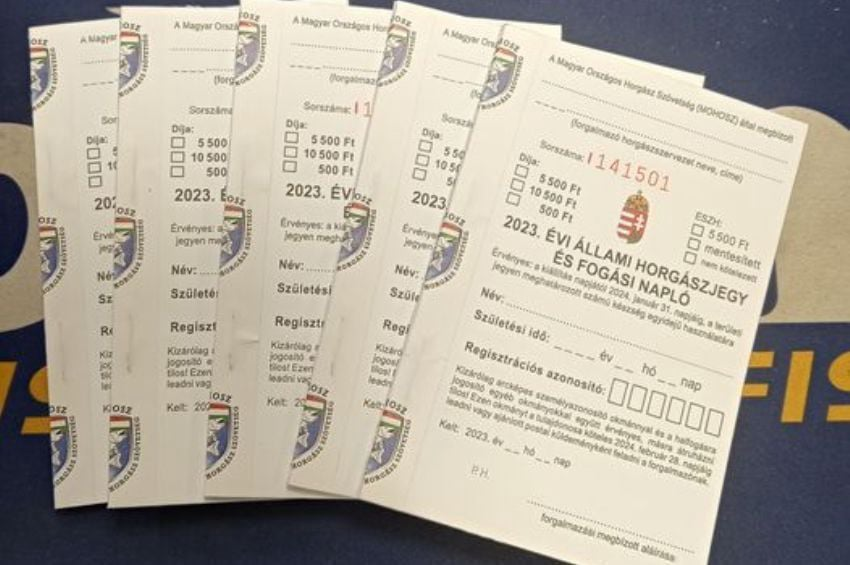
\includegraphics[scale=0.3]{images/fogasi_naplo.jpg}
\caption{2023. évi állami fogási naplók.}
\label{fig:fogasinaplok}
\end{figure}

Ezen a ponton találkozott a két kedvenc területem, a horgászat és a programozás. 
Az egyetemi éveim alatt szerteágazó tudásra tehettem szert, megismerhettem sokféle programozási nyelvet és
technikát. Külön kiemelném az adatbázis kezelést, és az objektum orientált programozási elvet, amelyek
nagy mértékben hozzásegítettek a szakdolgozati témám kiválasztásához, és megvalósításához.
Sokszor szó esett arról, hogy a programozás rengetegszer hétköznapi problémákat hivatott megoldani, ezáltal
könnyebbé tenni a felhasználó életét. 

Ezen a vonalon haladva határoztam el, hogy a szakdolgozati témám az állami fogási napló rendszer 
digitalizálása lesz. Ezzel az applikációval szeretném felhívni a figyelmet arra, hogy időleges
az előbbiekben említett rendszer átdolgozása, és a mai igényeket kielégítő okos telefonos integráció
létrehozása.

A továbbiakban be fogom mutatni, hogy az én elképzelésem alapján hogyan valósítható meg egy Androidos alkalmazás
Android Studio fejlesztői környezetben. Célja az alkalmazásnak, hogy felhasználó barát módon segítse horgásztársaimat a hétvégi kikapcsolódás során gyűjtött adatok - például a fogott halak súlya, a fogás pontos helye és időpontja - rögzítésére, és rendszerezésére. Az applikáció ezen túl segít a régebben rögzített fogások 
visszakeresésére, és áttekintésére. Kiemelt szempont volt az, hogy kezdő telefon felhasználók, ezáltal
az idősebb, okostelefont kevésbé használni tudók is könnyen és gyorsan használatba vehessék az alkalmazást. 
Törekedtem arra, hogy a program kezelői felülete a lehető legegyszerűbb, és átlátható legyen.

\begin{figure}[h]
\centering
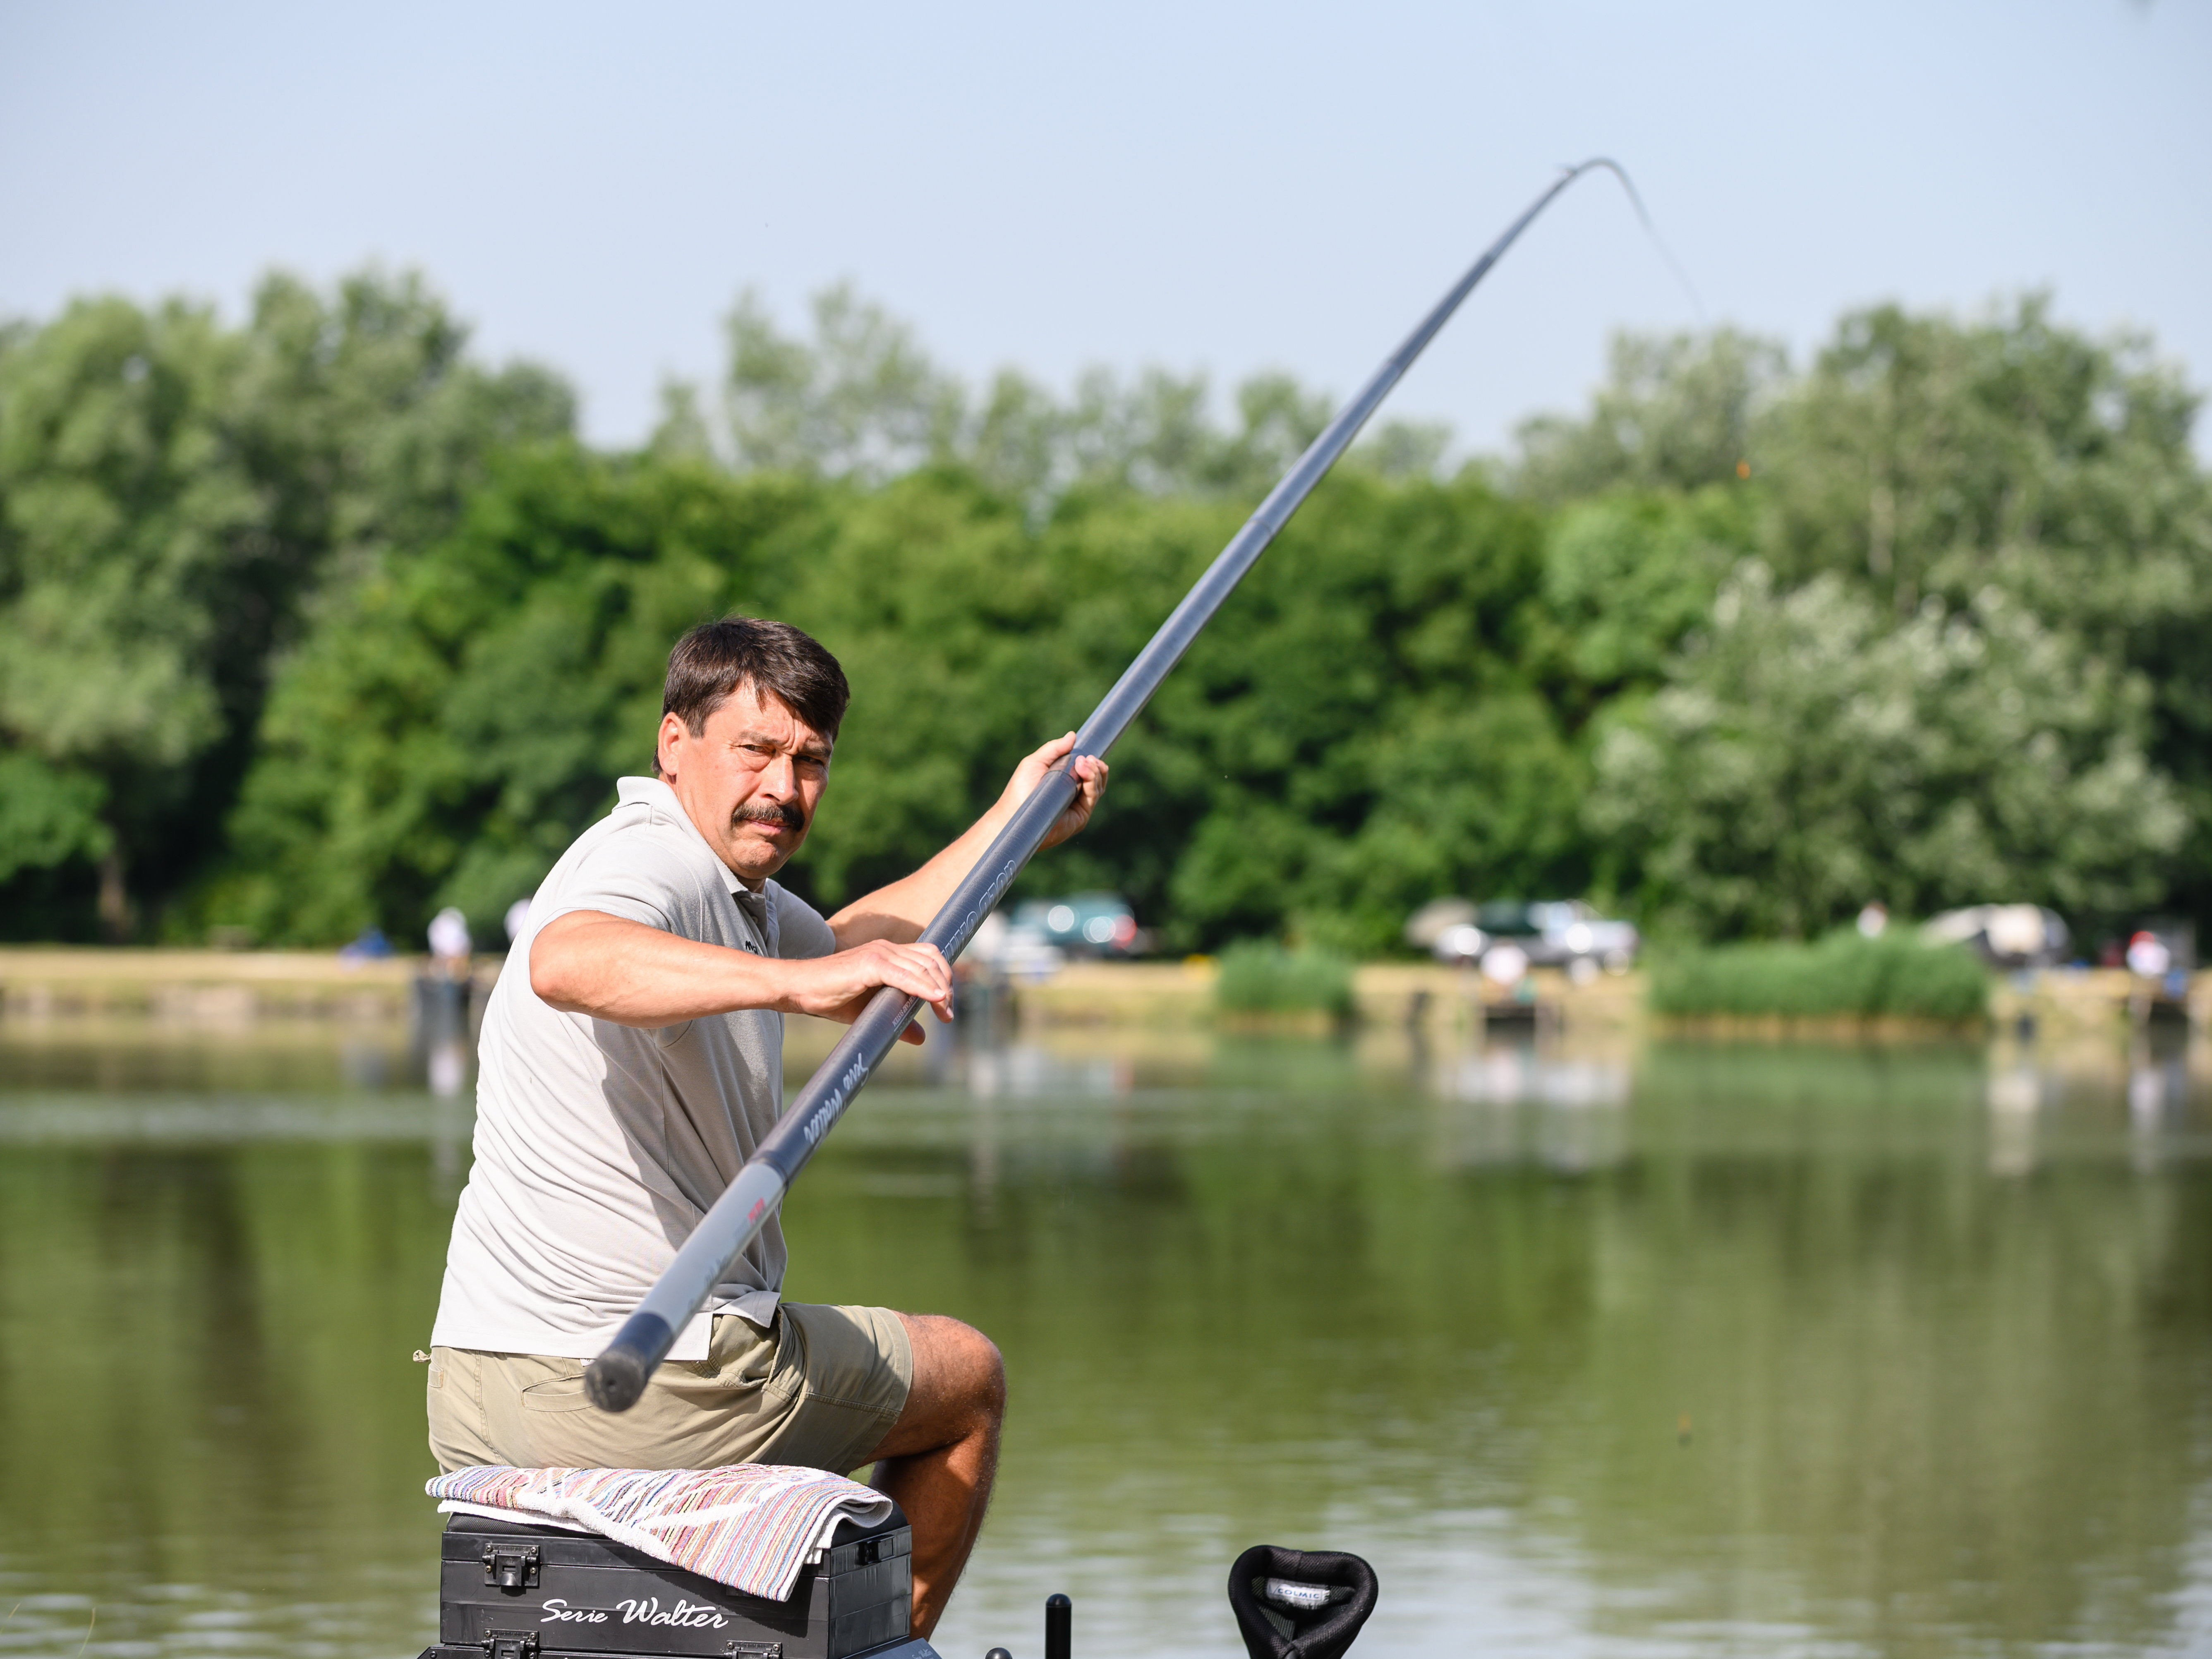
\includegraphics[scale=0.2]{images/horgaszat.jpg}
\caption{Horgászati tevékenységet végző ember.}
\label{fig:horgasz}
\end{figure}

A dolgozat az alábbi felépítést követi: az első fejezet bevezeti az olvasót a jelenlegi piaci helyzetbe, és 
rámutat a hiányosságokra, majd egy lehetséges megoldást nyújt. A második fejezet a fejlesztéshez szükséges 
technológiai alapokat, különösen az Android Studio és a hozzá kapcsolódó eszközök használatát mutatja be. A 
harmadik fejezet az alkalmazás architektúráját és a funkciók részletes leírását tartalmazza, míg a negyedik 
fejezet az alkalmazás megvalósításának módszereit tárgyalja. Az ötödik fejezet a tesztelési fázist mutatja be,
az utolsó fejezet pedig összefoglalja a projekt eredményeit, és javaslatokat fogalmaz meg a jövőbeni fejlesztésekre.
\chapter{A telefonos alkalmazás fejlesztés}

A bevezetőben említett probléma nem újkeletű, a MOHOSZ tisztában van a horgász fogási napló digitalizálásával
kapcsolatos felmerülő igényekkel, több próbálkozás is volt már, mindent átfogó megoldás azonban eddig még nem valósult meg, csak tervek vannak terítéken\cite{Mohosz}.

A telefonos alkalmazások fejlesztésére több különböző módszer is létezik, ebben a fejezetben szeretném
ezt részletesebben bemutatni.

\section{Különböző szoftverek bemutatása}

A telefonos applikációk fejlesztésére többféle platformon elérhető szoftverek léteznek.
Továbbiakban ismertetni szeretném a kifejezetten számítógépes platformra készített népszerűbb programokat,
amelyek a telefonos alkalmazás fejlesztést hivatottak megkönnyíteni.
\vspace{.5cm}

Az egyik legnépszerűbb választás a Flutter, ami a felhasználó számára lehetővé teszi, hogy egyszerre
fejlesszenek a két legnagyobb telefonos platformra, azaz Android-ra , és IOS-re (továbbiákban Cross-platform).
Ez egy DART keretrendszeralapú ˝widget˝ fejlszetést kínál, aminek az előnye a gyors User Interface készítés,
és széleskörű testreszabhatóság\cite{Flutter}. Készítője a Google.

\begin{figure}[h]
\centering

\includegraphics[scale=0.2]{images/flutter.png}
\caption{Flutter logó}
\label{fig:flutter}
\end{figure}

A másik népszerű választás a React Native\cite{React}, amely szintúgy egy Cross-platform alkalmazás készítő szoftver,
amelyet a Facebook fejlesztett ki. A program JavaScript, illetve TypeScript programnyelvet használ,
nagy hangsúlyt fektet a gyorsaságra.

\begin{figure}[h]
\centering

\includegraphics[scale=0.1]{images/reactnative.png}
\caption{React Native logó}
\label{fig:reactnative}
\end{figure}

Említésre méltó a Unity\cite{Unity}, amely kifejezetten játék fejlesztésre készült szoftver.
Többek között képes számítógépes, konzolos és telefonos alkalmazás fejlesztésre is.
Fejlesztési nyelve a C\#.

\begin{figure}[h]
\centering

\includegraphics[scale=0.12]{images/unity.png}
\caption{Unity logó}
\label{fig:unity}
\end{figure}

A következő alkalmazás az Xcode\cite{Xcode}, amely az Apple hivatalos fejlesztői környezete.
Ezzel a szoftverrel csak az Apple ökoszisztémán létező operációs rendszerekre tudunk fejleszteni,
azaz iOS, iPadOS, macOS, watchOS és tvOS. Fejlesztési nyelve a Swift, és Objective C.

\begin{figure}[h]
\centering
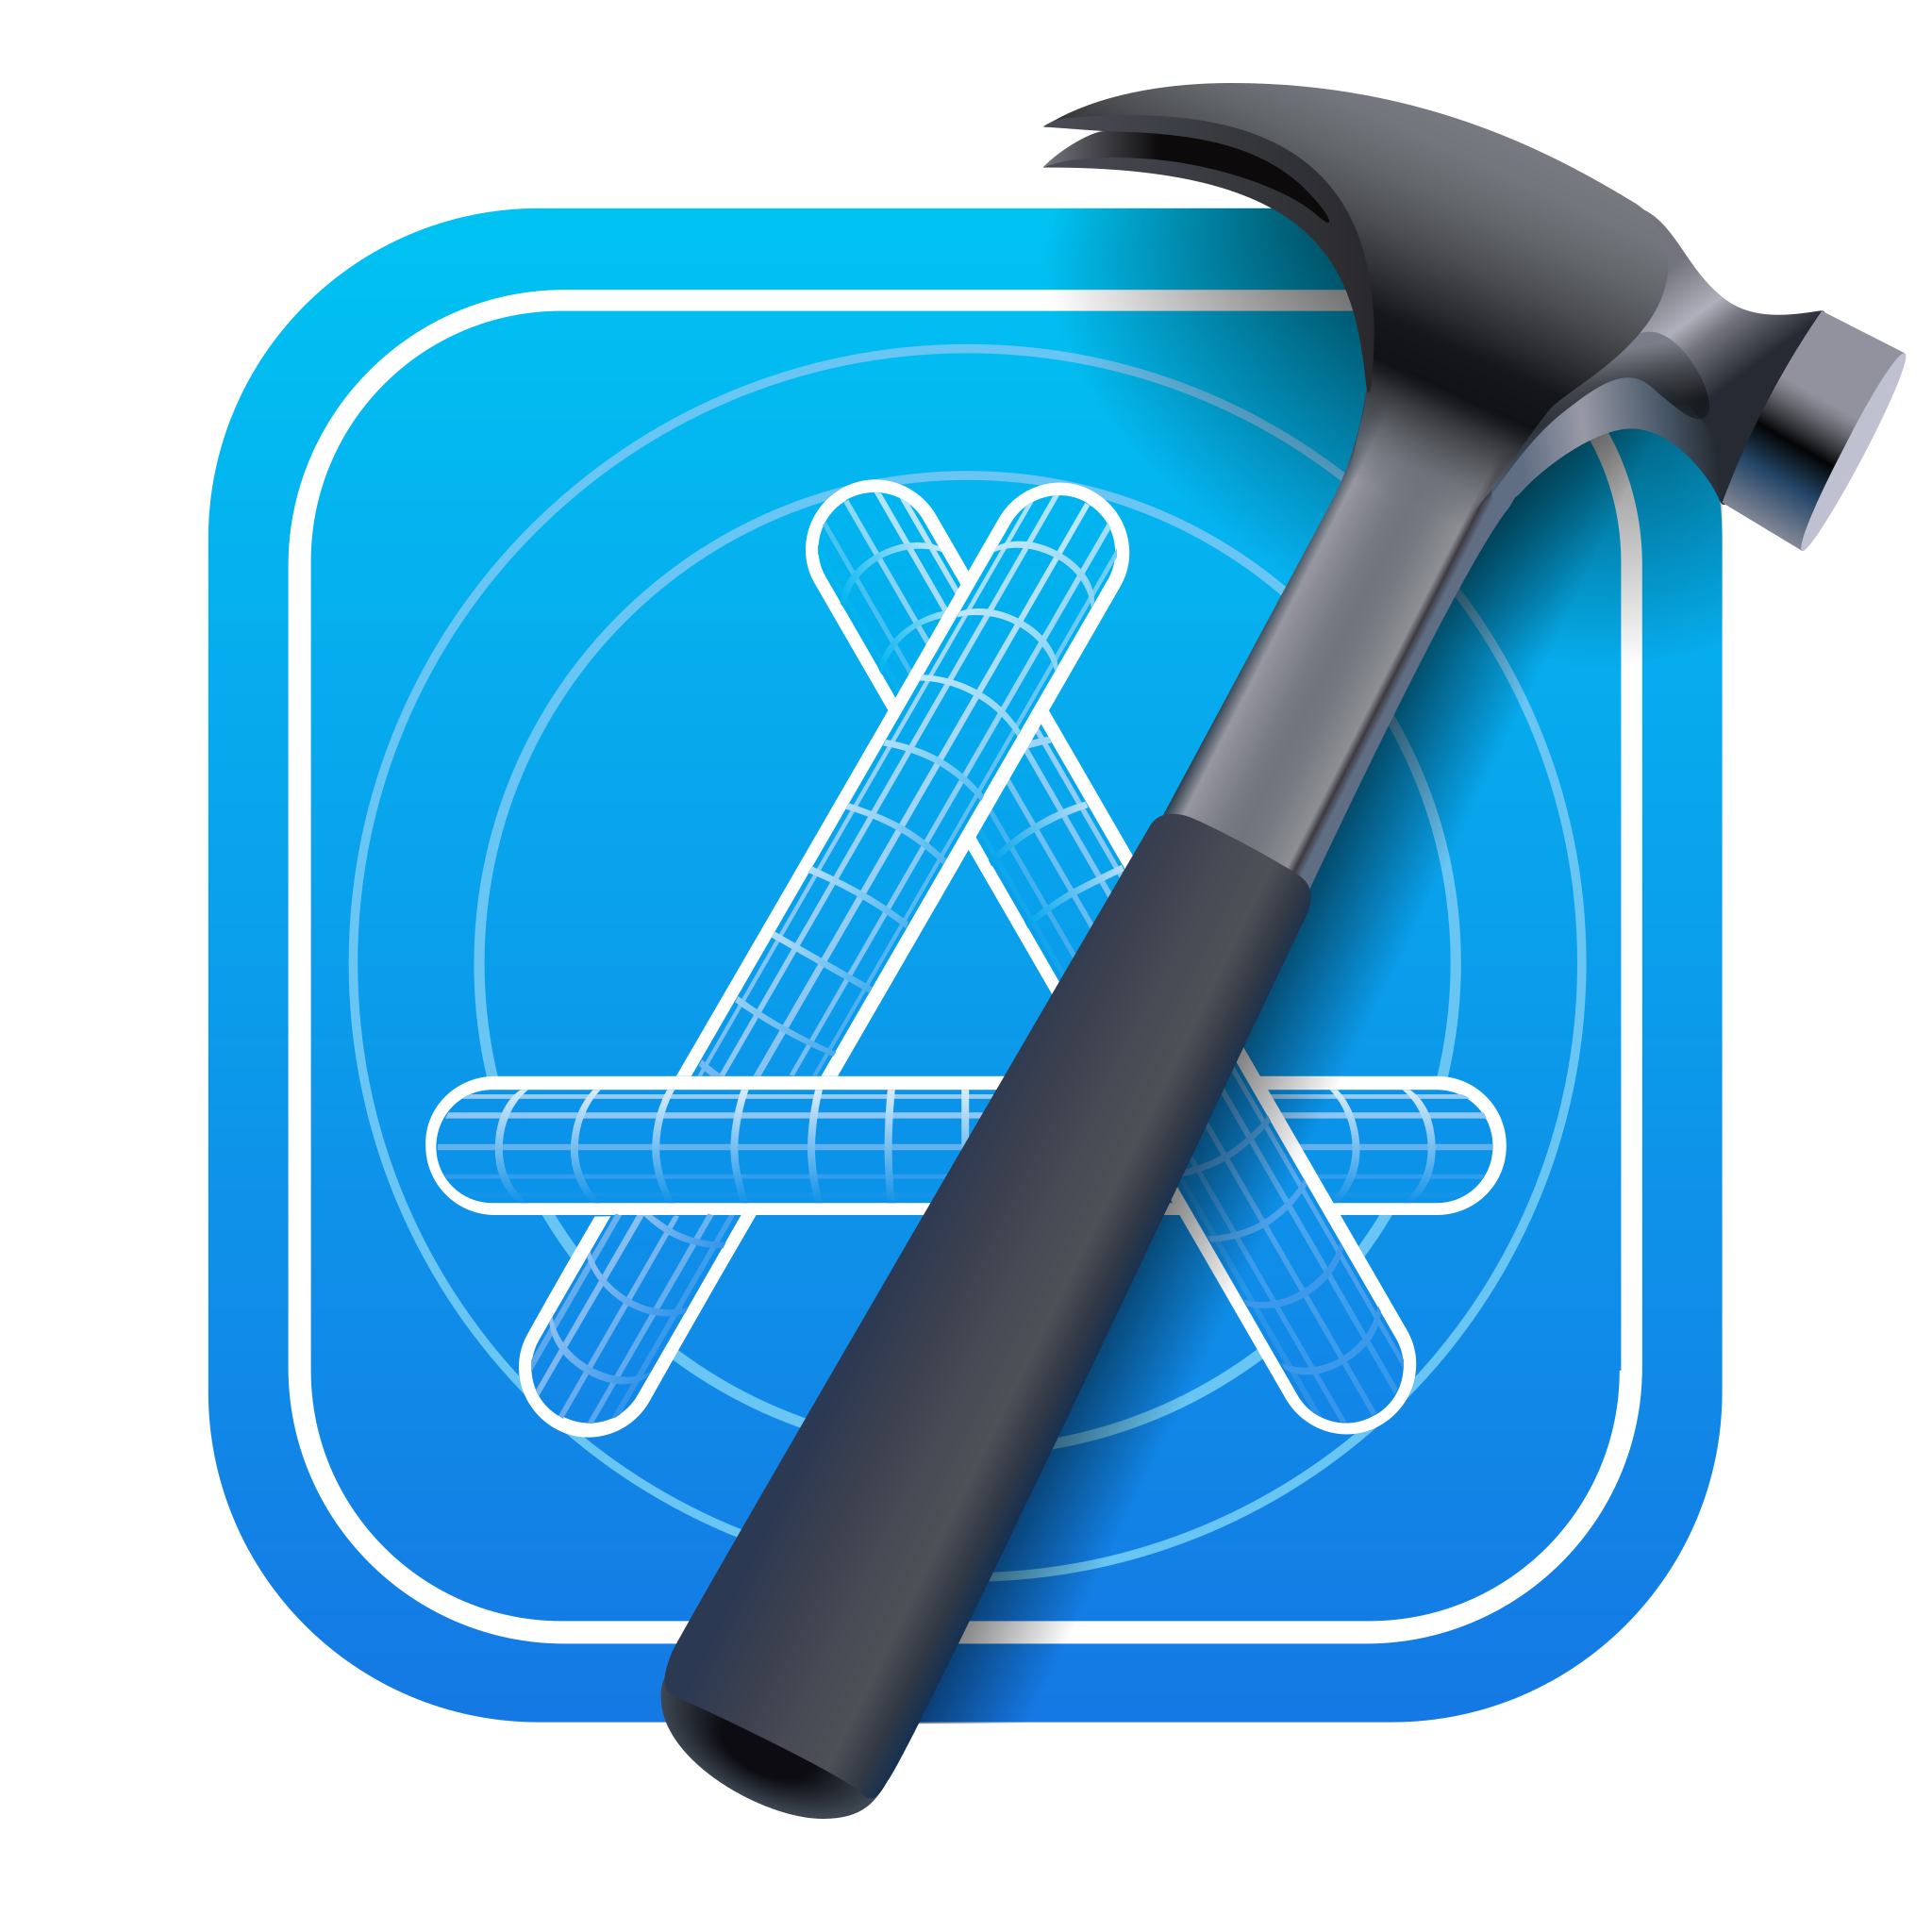
\includegraphics[scale=0.08]{images/xcode.png}
\caption{Xcode logó}
\label{fig:xcode}
\end{figure}

Utoljára pedig az általam választott szoftvert mutatnám be röviden, az Android Studio-t\cite{AndroidStudio}.
Ez a Google által fejlesztett hivatalos fejlesztő környezet, amellyel Andoridos alkalmazások
készítését teszik elérhetővé. Ez egy teljeskörő eszközkészlet, rendelkezik Android SDK-val, és 
beépített emulátorral, ami megkönnyíti a gyors tesztelést. Fejlesztési nyelve elsősorban a Kotlin, és a Java.

\begin{figure}[h]
\centering

\includegraphics[scale=0.08]{images/androidstudio.png}
\caption{Android Studio logó}
\label{fig:androidstudio}
\end{figure}

Az előbbiekben felsorolt fejlesztői környezeteknek nagyon sok előnye, és hátránya van. 
Az általam megadott szempontok a következők voltak: 
\begin{itemize}
    \item Androidon futtatható legyen az alkalmazás, hozzám közelebb áll a platform szemlélete a nyílt forráskódú applikációk terén.
    \item A fejlesztő környezet által használt nyelv sem elhanyagolható. Szerettem volna, ha egy magas szintű programozási nyelv lenne a használt az adott környezetben, tekintve hogy azokban szereztem a legtöbb tapasztalatom.
    \item Fontos volt a beépített emulátor, hogy az alkalmazásomat minél gyorsabban tudjam tesztelni.
    \item Nem utolsó sorban szerettem volna, ha az általam választott API-kat minél gördülékenyebben tudomm integrálni.
\end{itemize}

Ezen szempontok alapján haladva úgy döntöttem, hogy az Android Studio lesz számomra a legmegfelelőbb választás.

\section{Az Android Studio részletezése}

Az Android Studio a Google által készített hivatalos fejlesztőkörnyezet, amellyel natív 
Android alkalmazásokat tudunk készíteni.
A környezet a JetBrains IntelliJ IDEA\cite{Jetbrains} alapjaira épül, ebből lett tovább fejlesztve az Android platformra történő alkalmazások fejlesztésére.
Az Androidos platformon ez a legjellemzőbben használt IDE.


\begin{figure}[h]
\centering

\includegraphics[scale=0.08]{images/androiddev.png}
\caption{Android Developers logó}
\label{fig:androiddevelopers}
\end{figure}

Az Android Studio főbb funkciói, és jellemzői:
\begin{itemize}
    \item \textbf{Emulator:} A beépített emulátorral\cite{Emulator} a fejlesztés során gyorsan ki lehet próbálni az alkalmazáson eszközölt változtatásokat. Ezenkívül az emulatorral beállíthatjuk
    a tesztelni kívánt Android verziót, illetve készüléket, ezáltal tesztelni tudjuk alkalmazásunkat
    különböző verziószámú operációs rendszereken.
    \item \textbf{Build System (Gradle):} Az Android Studio Gradle-t\cite{Gradle} használ építési 
    rendszerként, amely megkönnyíti az alkalmazások automatizált építését és kezelheti a 
    különböző verziókat, függőségeket. A Gradle segítségével lehetőségünk van különböző
    buildek létrehozására, ami kulcsfontosságú volt a fejlesztés egyes fázisaiban.
    \item \textbf{Integrált hibakeresés és teljesítményelemzés:} A fejlesztői környezet lehetővé teszi, hogy könnyen diagnosztizáljuk és kijavítsuk az alkalmazásunk problémáit.
    Különféle eszközökkel, például CPU és memóriafigyelőkkel segít abban, hogy optimalizáljuk az alkalmazás teljesítményét.
    \item \textbf{Firebase és egyéb felhőszolgáltatások támogatása:} 
    Az Android Studio integrációt biztosít a Google Firebase platformmal\cite{Firebase}, ami megkönnyíti az
    adatbázisok, hitelesítés, felhasználói elemzések, értesítések és más felhőszolgáltatások 
    beépítését az alkalmazásba. Ez volt a legfontosabb szempont számomra, mivel az alkalmazásom több ponton is támaszkodik ezekre az API-kra.
    \item \textbf{Aktív közösség és támogatás:} A Google rendszeresen frissíti az Android Studiot, és nagy fejlesztői közösség\cite{AndroidDevGroup} is támogatja, ahol gyorsan választ kaphatunk a kérdéseinkre.
\end{itemize}

\section{Androidos alkalmazás fejlesztés}

Az előbbiekben részleteztem pár szempontot a fejlesztői környezettel kapcsolatban, azonban nem szeretném kihagyni azt sem, hogy milyen előnyei vannak az erre a platformra való fejlesztésnek közvetlenül.
A specifikus platform kiválasztás előnyei:
\begin{itemize}
    \item \textbf{Felhasználók aránya:} Magyarországon az Android operációs rendszerrel rendelkező eszközök piaci részesedése eléri a 80\% több független forrás szerint is.\cite{statistic1}\cite{statistic2}
    \item \textbf{Nyílt forráskód:} Az Android egy nyitottabb ökoszisztéma\cite{aosp}, nagyobb szabadságot kap a fejlesztő az alkalmazás funkcionalitásának, és megjelenítésének létrehozásában.
    \item \textbf{Költségek:} Az alkalmazás fejlesztése, feltéve hogy mi csinálunk mindent, nem kerül pénzbe. Ezalól nem kivétel a fejlesztői környezet használata, alkalmazásunk elérhetővé tétele, és karbantartása sem.
    \item \textbf{Pulikálás:} Az elkészült Androidos alkalmazást sokkal könnyebben tudjuk publikálni különböző áruházakban\cite{fdroid}, nem vagyunk rákényszerítve a telefon gyári alkalmazás áruházára.
\end{itemize}

Az Android platform legfőbb hátránya:

\begin{itemize}
    \item \textbf{Fragmentáció, kompatibilitási problémák:} Legfőbb hátránya a platformnak a megszámolhatatlan mennyiségű hardver, és képernyőméret kombinációk. Ezáltal alkalmazásunk fejlesztésekor nagy valószínűséggel gyártunk olyan hibákat, amelyek láthatatlanok voltak számunkra. Ezentúl különböző Android verziók eltérőek lehetnek mind funkciókban, és használható API-kban. Ezáltal a fejlesztés elhúzódhat, mivel a lehető legtöbb készüléket kell lefednünk az alkalmazásunkal, ami időigényes.
\end{itemize}

\chapter{Tervezés}

\section{Az alkalmazás fejlesztés bemutatása}

Az Androidos alkalmazás, vagyis az e-Horgásznapló egy Android operációs rendszeren futó, adat rögzítésre használatos alkalmazás. Célom az egyszerű, felhasználóbarát kezelőfelület, ahol a lehető legegyszerűbben rögzíteni tudja a horgász a kifogott hal adatait, és a fogás helyszínét.
Az alkalmazást Android Studio segítségével fogom elkészíteni Kotlin segítségével a könnyebb átláthatóság, és kevesebb boilerplate\cite{boilerplate} kód miatt. Az alkalmazásom a korábban használt Model-View-controller fejlesztési elv helyett az új Model-View-ViewModel architektúrát használja, ezáltal az alkalmazás jövő állóbb.


\section{Model-View-ViewModel}

Ahogy az előző szekcióban említettem az alkalmazásom a Model-View-ViewModel architektúrát alkalmazza. Ennek a mintának az a célja, hogy elkülönítse az alkalmazás logikai rétegeit, így egyszerűbb lesz a kód karbantarthatósága, és újra használása. Ebben különösen segítségünkre lesz a nemrég bevezetett Jetpack Compose, ami a régi XML elrendezést hivatott leváltani.

A MVVM-nek\cite{mvvm} három fő része van:
\begin{itemize}
    \item Model: Az adatokat, és a logikát tartalmazó réteg.
    \item View: A felhasználói felület.
    \item ViewModel: Köztes réteg, ez köti össze a Model-t, és a View-t. Feladata az adatok feldolgozása, és kezelése.
\end{itemize}

\begin{figure}[h]
\centering
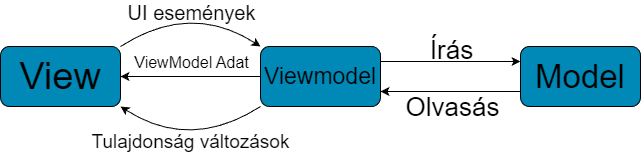
\includegraphics[scale=0.6]{images/mvvm2.png}
\caption{MVVM architektúra diagram}
\label{fig:mvvm}
\end{figure}

\subsection{Model}

A Model az alkalmazás adatait és üzleti logikáját tartalmazza. Ide tartoznak az olyan elemek, mint az adatbázisok, a hálózati API-k, vagy a fájlkezelés. A Model réteg az adatforrások elérését és az adatok frissítését biztosítja, de nem tartalmaz semmilyen logikát a felhasználói felülethez.

\subsection{View}

A View az a réteg, amely a felhasználói felületet kezeli. Ez felelős az adatok megjelenítéséért és a felhasználói bevitelek kezeléséért. A View réteg nem tartalmaz logikát az adatok feldolgozására; csak megjeleníti az adatokat, amelyeket a ViewModel szolgáltat számára.

\subsection{ViewModel}

A ViewModel az MVVM minta központi eleme, amely kommunikál a Model és a View között. A ViewModel adatokat kér a Modelltől, feldolgozza azokat, és úgy adja át a View-nak, hogy azok egyből megjeleníthetők legyenek. A ViewModel általában LiveData objektumokat használ, amelyek lehetővé teszik, hogy az adatok automatikusan frissüljenek a View-ban, ha változás történik bennük.

\section{A program felépítése}

A MVVM architektúra kulcsfontosságú szerepet fog betölteni az alkalmazásunkban. Mivel ezen szemlélet alapján kezdem el az alkalmazást, fontos hogy a \textbf{mindsk 21} (minimum Operációs rendszer követelmény) legyen beállítva. Ez jelen esetben az Android 5-ös verziót jelenti. 

A programban egyszerűségre törekszek, hogy minél szélesebb felhasználó közönség igénybe tudja venni a programot. Fontos, hogy intuitív, és letisztult legyen a kezelői felület, a lehető legkevesebb hibalehetőség merüljön fel a User részéről. Ezért a programom felépítését az alábbiak szerint képzelem el:

\begin{figure}[h]
\centering

\includegraphics[scale=0.6]{images/userdiagram.png}
\caption{felhasználói diagram}
\label{fig:userdiagram}
\end{figure}

A felhasználó az applikáció megnyitása után a bejelentkezés kijelzőre lesz irányítva, ahol be tud jelentkezni ideális esetben a MOHOSZ-nál regisztrált adataival. Miután ez megtörtént át lesz irányítva a fogási napló oldalra, ahol látni fogja az összes fogását időrendi sorrendben. 

\vspace{1cm}

Ezen a ponton tudja feltölteni a legfrissebb fogását a naplóba, ahol a következőket kell megadnia:
\begin{itemize}
    \item Tó neve
    \item Tó víztérkódja
    \item Hal neve
    \item Hal súlya
\end{itemize}

Ezután az alkalmazás automatikusan hozzárendeli a \textbf{SystemDate} változót, így elkerülve a különböző csalásokat, későbbi fogás hozzáadásokat a rendszerben. Tehát a felhasználó nem adhatja meg a fogásának az időpontját.

A fogás rögzítése után a rendszer hozzárendeli az adatbázishoz az éppen létrejött adatokat, és sorrend szerint legfelülre rakja. Itt megtekinthetjük a frissen hozzá adott fogást a régebben hozzáadotakkal együtt.

Ezen a ponton felmerülhet egy kérdés, hogy mi a helyzet akkor, hogyha úgy döntött egyik horgásztársunk, hogy a vízpartra mindenféle okos eszköz érkezik meg?
Itt jön szóba a fiók oldal, ahol ezt a problémát lenne érdemes orvosolni.

A fogási napló tetején egy \textbf{TopBar} változóval hozzárendelünk egy gombot, ami átvezet minket a fiók fülre, ahol megtekinthetjük az éppen bejelentkezett egyént, és felkínáljuk a lehetőséget a kijelentkezésre. Ezután az alkalmazás vissza vezet minket a bejelentkezés fülre, ahol sport társunk bejelentkezhet saját fiókjával, és nyomon követheti, illetve naplózhatja fogásait.

\subsection{Bejelentkezés}

Előszöri belépésnél a felhasználónak megoldást kell kínálni a bejelentkezéshez, amit nem lehet fél vállról venni. Minden alkalmazásban megadott adat szenzitív, alapos körültekintéssel kell ezeket kezelni. Mivel fejlesztő környezetnek az Android Studio-t választottam a különböző Google által fejlesztett API-k könnyen integrálhatóak az alkalmazásba. Ezt kihasználva hosszas tanakodás után a Firebase tűnik a legmegfelelőbb választásnak. 

A Firebase felhőszolgáltatást nyújt nekünk kölünböző előre létrehozott API-kal, amik gördülékenyebbé teszik az alkalmazás fejlesztés ezen szakaszát. Természetesen a bejelentkezésre is nyújt egy külön megoldást, aminek a neve \textbf{Firebase Authentication}\cite{firebaseauthentication}. Ezzel az API-val dolgozva csak meg kell adnunk a bejelentkezés típusát, és máris neki állhatunk az alkalmazásba való beépítésnek. Itt fontos megemlíteni, hogy ez a szolgáltatás nem teljesen ingyenes, csak egy bizonyos erőforrás kapacitás használatáig, azonban a mi esetünkben az alkalmazás méretét tekintve nem befolyásoló tényező.

A bejelentkezés a Firebase integrációja után így nézne ki:
\begin{itemize}
    \item E-mail beviteli mező
    \item Jelszó beviteli mező
    \item Bejelentkezés gomb
\end{itemize}

A bejelentkezés gomb megnyomása után ellenőrizni tudjuk, hogy a felhasználó által, vagy általunk által megadott bejelentkezési információk megegyeznek-e az adatbazisban szereplő értékekkel. 

\begin{figure}[h]
\centering

\includegraphics[scale=1]{images/login.png}
\caption{A bejelentkezés panel egy elképzelt változata.}
\label{fig:loginpanel}
\end{figure}

\subsection{A fogási napló}

Mituán bejelentkezett a User szeretném, ha egyből a fogási napló oldalon találná magát. 
Az alkalmazás elemi része továbbra is az egyszerűség, így a könnyű felhasználást szeretném ezzel elősegíteni. Mivel itt adatokat fogunk tárolni szükségünk van valamilyen adatbázisra.
Erre a célra az Android studio-ban integrált \textbf{Room}\cite{room} adatbázist fogom használni, ami egyszerűen lokálisan tárolja a felhasználó által feltölteni kívánt adatokat.
Ezen a ponton szeretném, ha sima felsorolás nézetben megtudja tekinteni a felhasználó az eddigi fogásait az alábba szempontok szerint:
\begin{itemize}
    \item Fogás időpontja
    \item Fogás helye
    \item A tó víztérkódja
    \item Hal típusa
    \item Hal súlya
\end{itemize}

A képernyő jobb alsó sarkában ésszerű lenne egy \textbf{FloatingActionButton}, ami az adatfelvitel \textbf{Dialog}-ra vezetne át minket, ahol feltölthetjük az adatainkat.

A fogás időpontja a korábban említett \textbf{Systemdate} változó lenne, amit nem tudunk megváltoztatni, mindig a fogás rögzítésének ideje szerepel.
A fogás helye természetesen a tó neve lenne, ami egy \textbf{String} változó, itt begépelhetjük az éppen kikapcsolódás céljával használatba vett vizet.
A tó víztérkódja nem elfelejthető adat, ez \textbf{Int} változó lenne.
A hal típusa, pontosítva a hal neve egy \textbf{String} változó lenne, ahogy megadhatjuk a fogott halunk nevét.
Végül a hal súlya értelemszerűen a mérlegelés után megállapított szám avagy \textbf{Int}, kilogramm-ban.

\subsection{Fiók}

Az utolsó szekció a fiók oldal, ami azt szolgálná, hogy a felhasználó ki tudjon jelentkezni az alkalmazásból, lehetőséget biztosítva egy másik fiók bejelentkezésére, vagy ugyanazzal az adatokkal való vissza-jelentkezésre.

Itt biztosítani kell a felhasználónak egy kijelentkezés gombot, amivel kijelentkezik a fiókjából, és visszatér a bejelentkezés oldalra. 

Továbbá egy másik lehetőséget is érdemes felkinálni a felhasználónak, ahol visszatud térni a fogási napló oldalra.
\chapter{Megvalósítás}

\section{Előkészület}

Mivelhogy Androidos alkalmazásom kezdeti része nagy mértkében hagyatkozik a Firebase által nyújtott szolgáltatásokra, fontos ezeket megvalósítani a program létrehozásának megkezdése előtt.
\begin{itemize}
    \item Először is szükségünk lesz egy Firebase regisztrációra.
    \item Sikeres regisztráció után létre kell hoznunk egy Firebase projektet, ami az alkalmazásunk felhő alapú szolgáltatásait hivatott megvalósítani.
\end{itemize}

Ezen a ponton érdemes létrehozni az Android Studio projectet, ugyanis a Firebase-nak szüksége van a project adataira a sikeren háttérszolgáltatások ellátásához.

Szükségünk lesz az Android Studio programra, ahol a munka nagy része zajlani fog.
Ezt a hivatalos weboldalról\cite{AndroidStudio} tudjuk ingyenesen beszerezni.
Ezután a programot fel kell telepíteni, majd használatba is vehetjük.
Miután beléptünk a programba, az első dolgunk egy új project létrehozása, amit a GUI-n keresztül a bal felső sarokban lévő \textbf{File>New project} útvonalon találunk meg.
Továbbiakban a projekt létrehozási képernyőre\ref{fig:newproject} leszünk irányítva, ahol kiválaszthatjuk programunk alapvető felépítését, avagy a vázát.

\begin{figure}[h]
\centering
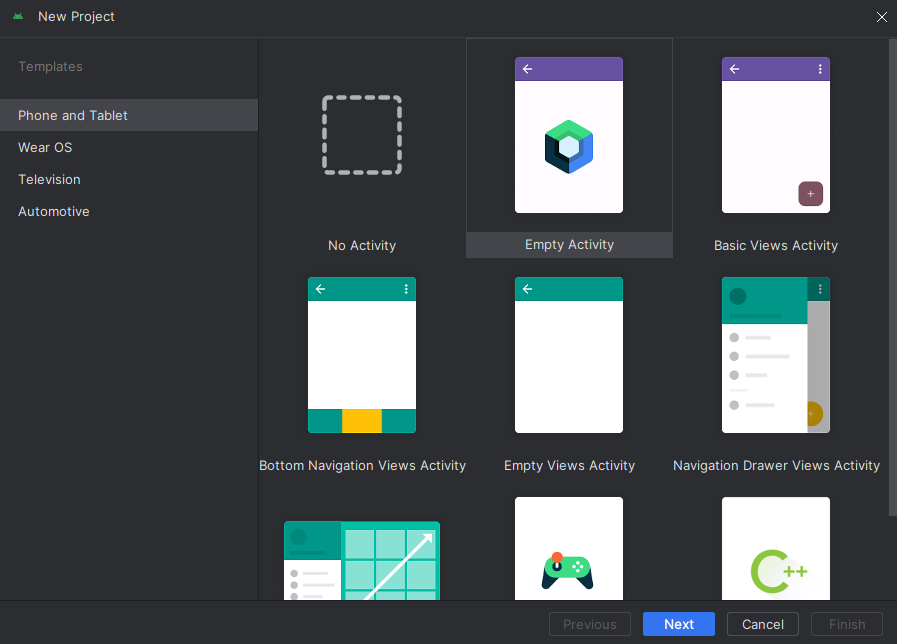
\includegraphics[scale=0.4]{images/android studio.png}
\caption{Projekt létrehozási ablak.}
\label{fig:newproject}
\end{figure}

Itt az IDE több lehetőséget is felkinál, én az \texttt{Empty Activity} sémát használom. Ebben a módban az Android Studio elkészíti nekünk az alap felépítését, függőségeit a programnak, ezáltal nekünk nem kell bajlódni a beállításokkal.
Ha ez megvan, akkor sikeresen létrehoztuk a projektünket az Android Studio keretein belül, ami biztosítja nekünk a futtathatóságot.

Miután létrehoztuk az Android Studio Projektet vissza kell mennünk a Firebase-en létrehozott projektünk oldalára, és hozzá kell rendelnünk a számítógépünkön létrehozott projekthez.
Ezt egész egyszerűen megtehetjük, a hozzáadásnál csak a gyökérkönyvtár nevét (esetünkben
\texttt{eu.thesis.onlinecatchlog}) kell megadni, ezzel elkezdtük a háttérszolgáltatás kiépítését.
Következő lépésként az Authentication fület lenyitva hozzá kell adnunk a projektünkhöz, majd bekapcsolni az E-mail, és jelszó alapú bejelentkeztetést. Ezután már csak annyi van hátra a Firebase Console-on belül, hogy létrehozunk egy teszt fiókot, amivel az alkalmazás fejlesztése közben tesztelni tudjuk majd a funkciók működését.
Ezután érdemes letölteni a Firebase által kínált \texttt{google-services.json} nevezetű fájlt, amit el kell helyeznünk a projekt mappába. Ezáltal a későbbiekben hozzáadott funkciók össze tudnak kapcsolódni a felhőben létrehozott adatokkal.

Ennek az elvégzése után térjünk vissza az Android Studio felületére, ugyanis a projektünkben még nem inicializáltuk a Firebase-t. Ezt érdemes még a fejlesztési szakasz elején megtenni, ugyanis a külső könyvtár segítségével fogunk hivatkozni például a bejelentkezési képernyőn bevitt adatokra.

\begin{figure}[h]
\centering
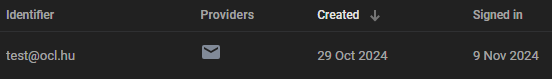
\includegraphics[scale=1]{images/firebaseloginadd.png}
\caption{A létrehozott tesztfiók.}
\label{fig:firebaseloginadd}
\end{figure}

A Firebase Console-ban további érdekes funkciókat is láthatunk, például használatra vonatkozó statisztikákat mutat ki, naplózza az alkalmazásunkhoz tartozó használati adatokat, amik nagyon fontosak a publikálás után. Így teljesebb képet kaphatunk a valós alkalmazás használati adatokról.

Mindezek után nyissunk egy terminált a projekt mappájában. Erre lehetőséget kínál közvetlen az Adnroid Studio is, így azt érdemes használni.

Projektünk még nem áll közvetlen összeköttetésben a szerverrel, ezért most inicializálni kell a Firebase-t a projekten belül.

A terminálba írjuk be a következőt:

\begin{verbatim}
    npm install -g firebase-tools
\end{verbatim}

Ezzel feltelepítjük a szükséges fájlokat a lokális szerver üzemeltetéséhez, amin belül tesztelni fogjuk az alkalmazásunkat.

Következőnok fontos, hogy az alkalmazás gyökérmappájába legyünk, használjuk az alábbi parancsot:
\begin{verbatim}
    firebase init
\end{verbatim}

Ezzel létrehoztunk a Firebase-nek szükséges fájlokat a projektünkben.
\begin{verbatim}
    firebase login
\end{verbatim}
Majd be kell jelentkeznünk a weboldalon megadott információkkal, hogy hitelesítsük magunkat.
\section{Android Studio projektek felépítése}

\subsection{Könyvtárak}

\textbf{Java/Kotlin könyvtár:} 
Itt található minden olyan fájl amely az alkalmazás fő logikáját hivatott megvalósítani.
Ezt hívjuk forráskódnak. A három fő csomag sorrendben \texttt{com.example.yourappname}. Ez a gyökércsomag, ami tartalmaz minden olyan Kotlin fájlt, amely elengedhetetlen alkalmazásunk futtatásához. Többet között itt található meg a korábban említett \textbf{MVVM} fájlok is.
Fontos kiemelni, hogy a régebbi architektúrát alkalmazó, legacy kódok másmilyen elrendezésűek.

\textbf{res könyvtár:}
Az alkalmazáshoz szükséges forrásokat itt találjuk, amik az olvashatóságot hivatottak megkönnyíteni, illetve a kódismétlést szeretnék minimalizálni. Minden olyan UI elemen megjelenített \textbf{String} vagy \textbf{kép}, vagy \textbf{ikon}-t itt kell deklarálni.
Ennek a könyvtárnak az előbbiek alapján három fő egysége van: 
\begin{itemize}
    \item \texttt{drawable}, ahol megadhatjuk a az alkalmazásunkban használatos képeket, vektorgrafikus elemeket.
    \item \texttt{values}, ahol deklarálhatjuk a különböző sűrűn előforduló stringeket, színeket, és stílusokat.
    \item \texttt{mipmap}, ahol pedig az alkalmazás ikonjait tudjuk beállítani.
\end{itemize}
Az itt megtalálható deklarációkra a fejlesztés következő szakaszaiban csak hivatkozni kell.
Ezekhez a forrás fájlokhoz mi is hozzáadhatunk változókat, sőt fontos is hogy minimalizáljuk a kód ismétlést.

\subsection{Gradle}

Itt kettő fő komponenst kell megkülönböztetni: a \texttt{projekt} szintű, és az \texttt{app} szintű gradle fájlokat. Az előbbi fájl tartalmazza a projektünk moduljainak beállítasait, itt állíthatjuk be a különböző Gradle és Android Plugin verziókat. Az utóbbi az érdekesebb számunkra, ugyanis itt állíthatjuk be a specifikus függőségeket, megadhatjuk a minimum Android verziót, illetve SDK verziót, nem utolsó sorban különböző külső könyvtárakat importálhatunk, amivel szélesíthetjük alkalmazásunk funkcionalitását, és megkönnyíthetjük a fejlesztés folyamatát.

\subsection{Manifest}

Ennek a fájlnak régebben sokkal nagyobb jelentősége volt, ugyanis minden egyes oldalt amit létrehoztunk innen tudtunk inicializálni, alapvető funkciókat beállítani. Az új MVVM architektúra használatával ennek a fájlnak lényegében annyi szerepe maradt számunkra, hogy innen indítjuk el az alkalmazásunkat megnyitáskor.
\newpage

\begin{java}[caption = {AndroidManifest.xml fájl egy részlete}]
<activity
    android:name=".MainActivity"
    android:exported="true"
    android:label="@string/app_name"
    android:theme="@style/Theme.ThesisExamples">
    <intent-filter>
  <action android:name="android.intent.action.MAIN"/>

  <category android:name="android.intent.category.LAUNCHER"/>
    </intent-filter>
</activity>
\end{java}

Ahogy az alábbi programkód részleten láthatjuk, a \texttt{MainActivity.kt} nevű fájlt inicializálni kell az \texttt{AndroidManifest.xml} nevezetű fájlban, ugyanis az alkalmazás indításakor itt kerül inicializálásra az első képernyő, ami jelen esetünkben a \texttt{MainActivity}. Ezt a beállítást az \texttt{<intent-filter>} változóval tudjuk megtenni, ahol a \texttt{<category android:name="android.intent.category.LAUNCHER"/>} beállítással megmondjuk a programnak, hogy ez a kezdőpont.

\section{Az alkalmazás létrehozása}

A projekt létrehozása után egy üres keretet kaptunk, ami futtatható, azonban sok minden nincs rajta. Miután az előkészületekben megteremtettünk minden előleges feltételt, hogy alkalmazásunkat el kezdjük fejleszteni, nincs más hátra mint a programozás.

\subsection{MainActivity.kt}

\begin{java}[caption = {MainActivity.kt fájl egy részlete}]
@AndroidEntryPoint
class MainActivity : ComponentActivity() {
    override fun onCreate(savedInstanceState: Bundle?) {
        super.onCreate(savedInstanceState)
        configureFirebaseServices()

        setContent { MainApp() }
    }

    private fun configureFirebaseServices() {
        if (BuildConfig.DEBUG) {
            Firebase.auth.useEmulator(LOCALHOST, AUTH_PORT)
            Firebase.firestore.useEmulator(
            LOCALHOST, FIRESTORE_PORT)
        }
    }
}
\end{java}

Ennél a fájlnál részletesebben kiszeretnék térni a szerkezetre, illetve a leírt kódra, mivel ez adja egy nagyon kritikus részét az alkalmazásunknak. Miután az \newline
\texttt{AndroidManifest.xml}-nél beállította az IDE ezt a kezdőpontot, itt kell inicializálnunk az alkalmazást, és a Firebase-t.
\begin{itemize}
    \item Az \textbf{@AndroidEntryPoint} annotiáció jelzi a Hilt számára, hogy ez az activity egy belépési pont, azaz injektálni kell a függőségeket, amik később kellenek az alkalmazás számára.
    \item A \textbf{MainActivity} osztály a \textbf{ComponentActivity}-t örökli, amely az Androidos fejlesztői környezet egy alapl Activity-je. Szerepe különösen fontos a későbbi \textbf{@Compose} annotációkban, ugyanis ez lesz felelős a képernyő frissítésének.
    \item \textbf{onCreate} metódus: ez az Activity életciklusának kezdő pontja. Itt inicializálódik az alkalmazás. Ebben a részben hívjuk meg a 
    \textbf{configureFirebaseServices()} függvényt, amely konfigurálja a lokális tesztelést.
    \item A \textbf{setContent} meghívásával beállítjuk a felhasználói felületet, aminek a motorja a \textbf{MainApp()}.
\end{itemize}

\subsection{MainApp.kt}

A \textbf{MainApp()} függvény az alkalmazás központi függvénye, fő komponense. Ebben a függvényben állítjuk be a témát amit előre meghatároztunk, illetve a navigációs keretet is itt inicializáljuk.
A témát (\textbf{OnlineCatchLogTheme}) amit ebben a blokkban kiválasztunk az összes navigációs komponensre alkalmazni fogjuk. Ez magában foglalja a színeket, és betűtípusokat, és az éjszakai módot is.

\begin{java}[caption = {MainApp.kt fő függvény leírása.}]
@Composable
fun MainApp() {
    OnlineCatchLogTheme{
    
    }
}
\end{java}

A NavHost függvénnyel meghívjuk a \textbf{notesGraph} funkciót, azonban előtte inicializálnunk kell.
Előbb létrehozunk egy \textbf{appState} objektumot, amely tartalmazza az alkalmazás használata során létrejött utolsó állapotot, avagy képernyőt. Ezután a \textbf{NavHost}-on belül beállítjuk a kezdőképernyőt, amely az esetemben a \textbf{SplashScreen}. Ez a képernyő egy betöltési indikátor, ami az alkalmazás első oldala. Ez a képernyő arra jó, hogy a felhasználó gyorsabbnak érezze az alkalmazás működését, ugyanis nem csak egy sima fekete kijelzőt lát, hanem animációt.

\newpage

\begin{java}[caption = {Navhost meghívása, beállítása.}]
Surface(color = MaterialTheme.colorScheme.background) {
        val appState = rememberAppState()

        Scaffold { innerPaddingModifier ->
            NavHost(
                navController = appState.navController,
                startDestination = SPLASH_SCREEN,
                modifier = Modifier.padding(
                    innerPaddingModifier)
            ) {
                notesGraph(appState)
            }
        }
    }
\end{java}

A \textbf{notesGraph} függvény egy navigációs grafikos struktúráját definiálja.
Itt határozzuk meg az elérhető képernyőket, és azok nevét.

Az elérhető képernyők listája:
\begin{itemize}
    \item  \texttt{SignInScreen}: Ez a bejelentkező kijelzőnk, a \texttt{SplashScreen} után az első, amit lát a User.
    \item  \texttt{SplashScreen}: Az alkalmazás elindítása után ez a kijelző hivatott kiküszöbölni a különböző inicializálások miatti lassabb futást. Egy animációt tartalmaz.
    \item  \texttt{AccountScreen}: A képernyő, amellyel kijelentkezhetünk az alkalmazásból, és visszatérhetünk a bejelentkezés képernyőre.
    \item  \texttt{CatchlogScreen}: A fő képernyője az alkalmazásnak. Itt tudjuk a korábban meghatározott módon feltölteni fogásainkat, és megtekinteni a korábban felvitt adatokat.
\end{itemize}

\begin{java}[caption = {Az egyik elérhető képernyő.}]
composable(SIGN_IN_SCREEN) {
    LoginView(openAndPopUp = {
    route, popUp -> appState.navigateAndPopUp(route, popUp) })
}
\end{java}

Az \textbf{openAndPipUp} függvény a navigáció kezelésére szolgál az alkalmazásban.
Ez a kód minden lehetséges \textbf{View}-ban szerepel, ugyanis ezzel navigáljuk át a felhasználót a másik kijelzőre, miközben a stack-ből töröljük az előző képernyőt.
Ebben az esetben a \textbf{route} adja meg annak a képernyőnek a nevét, amelyre navigálni szeretnénk.
Fontos, hogy az appState-hez kapcsolódik, amelyben a függvényt az 
\newline
\textbf{appState.navigateAndPopUp} hívja meg. Ez biztosítja, hogy az appState megfelelően kezelje a navigációs műveleteket az alkalmazás különböző képernyői között.

\newpage

\section{SplashScreen}

Ebben a szekcióban láthatjuk először, hogy gyakorlatilag mi is az az MVVM. A \textbf{SplashViewModel} adja a logikai függvényeket, a \textbf{SplashView} pedig a megjelenítésért felelős.
Nézzük meg először a \textbf{SplashViewModel}-t.

\begin{java}[caption = {A SplashViewModel annotációja, és osztály definíciója}]
@HiltViewModel
class SplashViewModel @Inject constructor(
    private val accountService: AccountService
) : MainAppViewModel() {

}
\end{java}

\begin{itemize}
    \item @HiltViewModel: Ez az annotáció jelzi a Dagger Hilt-nek, hogy ez az osztály egy ViewModel. Ezután a Hilt keretrendszer automatikusan gondoskodik a különbözű függőségek injektálásáról.
    \item A SplashViewModel örökli a MainAppViewModel osztályt, ahol egy alap hibaelhárító függvény van jelen, a launchCatching. Ez minden ViewModel-nek a része.
    \item Az accountService egy privát függőség, amelyet a Hilt injektál a SplashViewModelbe.
    Ez a függőség az, amely kezeli az aktuális felhasználói fiók állapotát. Tehát ha a felhasználó be van jelentkezve, akkor nem szabad mégegyszer felkínálni neki erre a lehetőséget, hanem a főoldalra kell irányítani. Ellenkező esetben pedig a bejelentkező képernyőt kell neki felajánlani.
    
\end{itemize}

\begin{java}[caption = {onAppStart függvény deklarációja.}]
fun onAppStart(openAndPopUp: (String, String) -> Unit) {
    if (accountService.hasUser()) openAndPopUp(
    CATCHLOG_SCREEN, SPLASH_SCREEN)
    else openAndPopUp(
    SIGN_IN_SCREEN, SPLASH_SCREEN)
}
\end{java}

\section{LoginScreen}

Ez a screen teljes mértékben kihasználja a Model-View-ViewModel adta tulajdonságokat.
Ennek az oldalnak a bemutatását a Model felől közelíteném meg.

\subsection{AccountService}

Egy interfész, amely a felhasználói fiókkezelési műveleteket definiálja. Eme interfész segítségével a felhasználók ki, és be jelentkezhetnek.

\begin{itemize}
    \item \texttt{currentUser: Flow<User?>}: Egy Flow, amely nem összehangolt módon figyeli az aktuális felhasználói fiókot, és folyamatosan frissíti az adatokat, ha a felhasználó állapota megváltozik. A Flow hasonlóan működik mint egy lista, azonban itt az idő függvényében változik a lekérdezésre adott válasz.
    \item \texttt{currentUserId: String:} A jelenlegi bejelentkezett felhasználó azonosítója.
    \item \texttt{hasUser(): Boolean:}: Ellenőrzi, hogy van-e bejelentkezett felhasználó.
    \item \texttt{signIn(email: String, password: String):} Egy függvény, amely bejelentkezést hajt végre a megadott email és jelszó alapján.
    \item \texttt{signOut()}: Kijelentkezteti a jelenlegi felhasználót
\end{itemize}

\begin{java}[caption = {AccountService.kt}]
    interface AccountService {
    val currentUser: Flow<User?>
    val currentUserId: String
    fun hasUser(): Boolean
    suspend fun signIn(email: String, password: String)
    suspend fun signUp(email: String, password: String)
    suspend fun signOut()
}
\end{java}

\subsection{AccountServiceImpl}

Az AccountServiceImpl az AccountService interfész implementációja.A Firebase hitelesítési szolgáltatásait használja a felhasználói bejelentkeztetés megvalósítására.

A fontosabb funkciók, kiegészítve az előző szekcióban leírtakat:
\begin{itemize}
    \item \texttt{currentUser:} A callbackFlow-t használja, hogy folyamatosan figyelje a Firebase hitelesítési állapotát. Az AuthStateListener figyeli, ha a felhasználó állapota változik (pl. bejelentkezés vagy kijelentkezés), és frissíti a currentUser értékét.
    \begin{java}
override val currentUser: Flow<User?>
get() = callbackFlow {
    val listener =
        FirebaseAuth.AuthStateListener { auth ->
            this.trySend(auth.currentUser?.let {
                User(it.uid) })
        }
    Firebase.auth.addAuthStateListener(listener)
    awaitClose {
        Firebase.auth.removeAuthStateListener(listener) }
}
    \end{java}
    \newpage
    \item \texttt{crrentUserId}: Ez kérdezi le a jelenlegi felhasználó azonosítóját.
    \begin{java}
override val currentUserId: String
get() = Firebase.auth.currentUser?.uid.orEmpty()
    \end{java}
    \item \texttt{hasUser()}: Megvizsgálja, hogy a Firebase.auth.currentUser értéke nem null, ami azt jelenti, hogy van bejelentkezett felhasználó. Ha null, akkor értelemszerűen jelenleg nincsen bejelentkeztetett user.
    \begin{java}
override fun hasUser(): Boolean {
return Firebase.auth.currentUser != null
    }
    \end{java}
    \item \texttt{signIn(email, password)}: Aszinkron módon bejelentkezteti a felhasználót az email és password paraméterek alapján.
    \begin{java}
override suspend fun signIn(
email: String,
password: String) {
    Firebase.auth.signInWithEmailAndPassword(
    email, password).await()
}
    \end{java}
    \item \texttt{signOut()}: Kijelentkezteti a felhasználót a Firebase hitelesítési rendszerből.
    \begin{java}
override suspend fun signOut() {
Firebase.auth.signOut()
}
    \end{java}
\end{itemize}

\subsection{LoginViewModel}
Ez előbbiekben felsorolt funkciók elemi részét képezik ennek a program blokknak. A LoginViewModel lesz az az elem, ami összeköti a Model-eket a View-al, azaz információt szolgáltat a felhasználónak.
Kezdjük a függőségekkel:
\begin{itemize}
    \item \texttt{AccountService}: Ez felelős a felhasználói bejelentkeztetésért. A LoginViewModel ezt használja a \texttt{signIn} meghívásával a bejelentkezési folyamat elindításához.
    \item  \texttt{@Inject constructor}: Ennek a módszernek a segítségével állítjuk elő az AccountService példányt a LoginViewModel számára.
\end{itemize}
Található továbbá kettő darab \textbf{MutableStateFLow}, amellyel az állapotfolyamatok, és az értékek frissítésést teszi lehetővé. A Composse automatikusan újra rajzolja a felhasználói felületet, ha ezek a \textbf{StateFlow}-k frissülnek.

Ezen felül a legfőbb függvény ebben a blokkban az \texttt{onSignInClick}.
Itt lesz kulcsfontosságú a korábban említett \texttt{openAndPopUp}, ugyanis itt csatolunk vissza a \textbf{MainApp}-ban lévő navigálási komponensre. Először a \texttt{route}-al megnevezzük a célképernyőt, amelyre át szeretnénk irányítani a User-t sikeres bejelentkezés után. Másdszor pedig a \texttt{popUp} változóval eltávolítjuk a navigációs stack-ből a jelenleg használt képernyőt. Ez azért fontos, mert a felhasználó így nem tud a telefonján a visszalépéssel visszatérni a bejelentkező panel-ra, hanem az alkalmazásból fog kilépni.
\begin{java}[caption = {onSignInClick függvény.}]
fun onSignInClick(openAndPopUp: (String, String) -> Unit) {
    launchCatching {
        accountService.signIn(email.value, password.value)
        openAndPopUp(CATCHLOG_SCREEN, SIGN_IN_SCREEN)
    }
}
\end{java}

\subsection{LoginView}
Ezzel elérkeztünk az oldal megjelenítő részéhez. Az itt deklarált függvények, metódusok, változók felelősek azért, hogy a megjelenített tartalom pontosan ott legyen ahol szeretnénk.

Kezdjük itt is a függvényparaméterekkel:
\begin{itemize}
    \item \texttt{modifier: Modifier}: Ez egy alapértelmezett paraméter, amellyel lehetővé 
    \newline
    tesszük a komponensek vizuális, és elhelyezési tulajdonságainak módosítását. Legtöbbet a méretezésre, és az elhelyezésre használtam.
    \item \texttt{viewModel: LoginViewModel}: Ezzel a származtatással férünk hozzá a 
    \newline
    LogInViewModel-ben deklarált bejelentkezési logikához és állapotokhoz. 
    \newline
    A \texttt{hiltViewModel()} miatt a Hilt automatikusan injektálja, így megkapjuk az állapotokat és műveleteket.
\end{itemize}

Következő fontos blokkunk az állapotgyűjtés. Amikor a felhasználó használatba veszi a e-mail és password mezőt, akkor a képernyőt frissíteni kell minden alkalommal. Tehát ezek a \textbf{State} objektumok felelősek a komponensünk újra rajzolásáért.

\begin{java}[caption = {E-mail, és jelszó State objetumok.}]
val email = viewModel.email.collectAsState()
val password = viewModel.password.collectAsState()
\end{java}

Számomra az egyik legnagyobb nehézséget a Jetpack Compose használata jelentette, ugyanis ez a 
fajta UI szemlélet nagy mértékben eltér a korábban használt Activity/Fragment felépítéstől.

Ennek a fajta UI felépítésnek ezek a főbb egységei:
\begin{itemize}
    \item \texttt{Column}: Ez fedi le a teljes bejelentkezési kijelzőt. Ezzel azt dekraláljuk, hogy az elemek függőleges elrendezkedésben fognak szerepelni a kijelzőn.

    A \texttt{fillMaxWidth()} és \texttt{fillMaxHeight()} komponensekkel megmondjuk a
    \newline
    Column-nak, hogy a képernyő teljes egészét ki kell tölteni. Ezáltal az ebben a blokkban szereplő elemek a képernyő közepére kerülnek.

    A \texttt{verticalScroll(rememberScrollState())} -el görgethetővé tesszük a tartalmat, ezáltal ha az Androidos készülék amin használni tervezzük az alkalmazást nem rendelkezik elég nagy képernyőmérettel, vagy felbontással ugyanúgy megtudja jeleníteni a tartalmunkat.

    \item \texttt{Spacer}: Komponens elválasztóként működik, két elem közé beszúrva távolságot tudunk teremteni.

    \item \texttt{OutlinedTextField}: A bejelentkezési mezőket ezzel valósítottam meg. Az elején deklarálni tudunk pár fontos jellemzőt, amivel testreszabhatjuk ezt a blokkot.

    \begin{itemize}
        \item \texttt{singleLine = true} lényege, hogy a mező egyetlen soros lesz.
        \item \texttt{modifier.padding()} változóval margókat adunk a mezőhöz.
        \item \texttt{value = email.value} esetében az e-mail aktuális értékét jelenítjük meg.
        \item \texttt{onValueChange = { viewModel.updateEmail(it) }}
        
        a \texttt{viewModel.updateEmail()} meghívásával frissíti az e-mailt, amikor a felhasználó begépeli az adatait.
        \item \texttt{placeholder} egy alap szöveget ír ki amíg nem történik gépelés, ezzel is segítve a felhasználó tájékozódását a képernyőn.
        \item \texttt{leadingIcon} pedig hasonló módon megjelenít egy ikont, ami intuitívabbá teszi a kijelzőt.
    \end{itemize}
\end{itemize}

\begin{java}[caption = {Az OutlinedTextField szemléltetése.}]
OutlinedTextField(
        singleLine = true,
        modifier = modifier
            .fillMaxWidth()
            .padding(16.dp, 4.dp),
        colors = TextFieldDefaults.colors(
            focusedContainerColor = Color.Transparent,
            focusedIndicatorColor = Color.Transparent,
            unfocusedIndicatorColor = Color.Transparent,
        ),
        value = email.value,
        onValueChange = { viewModel.updateEmail(it) },
        placeholder = { Text(stringResource(R.string.email))},
        leadingIcon = { Icon(
            imageVector = Icons.Default.Email,
            contentDescription = "Email") }
        )
\end{java}
\newpage
\begin{itemize}
    \item \texttt{Button}: Értelemszerűen a bejelentkezési gomb, egyben az utolsó elem a 
    \newline
    LoginView-ban. Ennek a legfontosabb funkciója az \texttt{onClick()}. Amikor a felhasználó rákattint a gombra a ViewModel-ben meghívjuk az \texttt{onSignInCLick()}-et.
    Ez a függvény megpróbálja bejelentkeztetni a felhasználót a korábban megadott adatok alapján. Ha a bejelentkezés sikeres a ViewModel segítségével meghívjuk az \texttt{openAndPopUp}-ot, amely átnavigál minket a CatchLogScreen-re.
\end{itemize}


\begin{java}[caption = {A Button szemléltetése.}]
Button(
         onClick = { viewModel.onSignInClick(openAndPopUp) },
        modifier = modifier
            .fillMaxWidth()
            .padding(16.dp, 0.dp)
    ) {
        Text(
            text = stringResource(R.string.sign_in),
            fontSize = 16.sp,
            modifier = modifier.padding(0.dp, 6.dp)
        )
    }
\end{java}

\begin{figure} [h]
    \centering
    
\includegraphics[width=0.5\linewidth]{images/login.png}
    \caption{Az elkészült Login panel.}
    \label{fig:finishedlogin}
\end{figure}

\section{OnlineCatchLog}

Ebben a szekcióban is a Model részletezésével kezdeném. Itt részletezni fogom a háttérfolyamatokat, amik lehetővé teszik az adatbázisom működését.
\subsection{Model}
\begin{itemize}
    \item \texttt{CatchLogDao}: A \textbf{@Dao} annotációval ellátott CatchLogDao egy Data Acces Object\cite{dao}, amely az adatbázisom műveleteit kezeli. Itt látjuk a metódusokat, amelyen keresztül kommunikálunk a Room adatbázissal.
    
\newpage
    
    \begin{java}[ caption = {CatchLogDao.kt részlet.}]
    @Dao
    interface CatchLogDao{
    
    }
    \end{java}
    \begin{itemize}
        \item \texttt{@Upsert}: Ez a metódus felelős azért, hogy egy új fogást rögzítsünk az adatbázisban. Másodlagosan ellenőrzi a meglévő rekordokat is.
\begin{java}
@Upsert
fun upsertCatchLog(catchLog: CatchLog)
\end{java}
        \item \texttt{@Query}: Az alábbi lekérdezéssel elérjük az összes eddig felvitt fogást az adatbázisban. Fontos, hogy ez a lekérdezés időrendi sorrendben valósul meg, azaz mindig a legfrissebb fogás lesz legfelül.
\begin{java}
@Query("SELECT * FROM catchlog ORDER BY catchTime ASC")
fun getLogsOrderedByTime(): Flow<List<CatchLog>>
\end{java}
    \end{itemize}

    \item \texttt{CatchLogEvent}: Ez a zárt interfész tartalmazza az eseményeket, amelyet az alkalmazás különböző részei felhasználhatnak az események kezelésére.
    Minden esemény külön adat osztályként, vagy objektumként van. Ezekkel tudunk az eseményekre reagálni.
    \begin{itemize}
        \item A \texttt{SaveCatchLog} esemény akkor hasznos, amikor frissen el szeretnénk menteni egy új kitöltött fogást.
        \item A \texttt{setLakeName, setLakeCode, setFishName, set FishWeight} pedig az adatmezőket frissítik.
        \item A \texttt{ShowDialog} illetve \texttt{HideDialog} a fogás felvitelét elindító folyamat részei. Amikor a képernyőn rá kattintunk az új fogás felvitelére ezen eseményekkel dolgozunk.
        \item A \texttt{SortLogs} eseménnyel pedig beállíthatjuk az adatbázis lekérdezésének típusát, sorrendjét.
        
\begin{java}[caption = { A CatchLogEvent eseményei. }]
sealed interface CatchLogEvent {
object SaveCatchLog
data class setLakeName(val lakeName: String)
data class setLakeCode(val lakeCode: Int)
data class setFishName(val fishName: String)
data class setFishWeight(val fishWeight: Int)
object ShowDialog
object HideDialog
data class SortLogs(val sortType: SortType)
}
\end{java}
    \end{itemize}
    \item \texttt{CatchLogDataBase}: Ezen a ponton viztosítjuk a Room adatbázis konfigurcióját.
    Először a \textbf{@Database} annotációval létrehozzuk az adatbázist. Ennek a feladata, hogy kezelje a CatchLog entitásokat, azaz a felvinni kívánt fogásokat. Ez az entitás magában foglalja a korábban említett adatokat, azaz a tó nevét, víztérkódját, hal nevét, súlyát, és a fogás időpontját. Ebben az osztályban továbbá megtalálható egy metódus, az \texttt{abstract val dao: CatchLogDao}. Ez biztosítja a hozzáférést a korábban említett \texttt{CatchLogDao} interfészhez, amellyel az alkalmazás a műveleteket fogja végrehajtani az adatbázison.

\begin{java}[caption = {CatchLogDataBase osztálya.}]
    @Database(
    entities = [CatchLog::class],
    version = 1
)
abstract class CatchLogDataBase: RoomDatabase() {
    abstract val dao: CatchLogDao
}
\end{java}
    \item \texttt{DataBaseModule}: Ez egy Dagger Hilt modul, amely biztosítja az adatbázist az egész alkalmazás számára. Itt részletezni szeretném a különböző komponenseket:
    \begin{itemize}
        \item \texttt{@Module} és \texttt{@InstallIn(SingletonComponent::class)} annotációk biztosítják azt, hogy a \texttt{DatabaseModule} globális függőségekkel segítse az alkalmazás többi elemét, és hogy hozzáférhező legyen az alkalmazás futása alatt.
        
\begin{java}[caption = {DataBaseModul-ban szereplő annotációk.}]
@Module
@InstallIn(SingletonComponent::class)
\end{java}

        \item \texttt{@Provides}: Ez a függőség segít létrehozni az adatbázist, amelyet később az alkalmazás az futása alatt használhat. Itt sajnos használnom kellett a \texttt{allowMainThreadQueries} metódust, ugyanis másképpen hibát produkált az alkalmazás. Ezt a későbbiekben fontos lenne kiküszöbölni, ugyanis az adatbázis így a fő processzor szálakon fut, ami a teljesítményünket negatív irányba eltolja. Ideális esetben ez a folyamat a háttérszálakon futna.
\begin{java}[caption = {provideCatchLogDataBase függőség.}]
@Provides
fun provideCatchLogDatabase(
@ApplicationContext context: Context):
CatchLogDataBase {
    return Room.databaseBuilder(
        context,
        CatchLogDataBase::class.java,
        "catch_log_database"
    ).allowMainThreadQueries().build()
}
\end{java}
        \item A \texttt{provieCatchLogDao} pedig elérhetővé teszi az alkalmazás többi részének az \texttt{CatchLogDao}-hoz való szükséges hozzáféréseket.
\begin{java}
@Provides
    fun provideCatchLogDao(
    database: CatchLogDataBase): CatchLogDao {
        return database.dao
    }
\end{java}
    \end{itemize}
    \item Végezetül pedig van egy egyszerű enum típusunk, a \texttt{SortType}. Ebben az Enum-ban deklarálhatunk új rendezési típusokat, ez jelen esetben csak az idő alapú Sort, azonban ez később könnyen bővíthető köszönhetően a felépítésnek.
\end{itemize}

\subsection{CatchLogViewModel}

Itt a programkód elején 2 fontos annotáció található. Az egyik a \texttt{@OptIn}, amellyel lehtővé tesszük az alkalmazás számára, hogy kísérleti fázisban lévő funkciókat használjunk. Ez ebben az esetben a \texttt{flatMapLatest}, és a \texttt{stateIn}. Ezek a funkciók az adat áramlásra, és az állapotkezelésre vonatkoznak.

A másik a \texttt{@HiltViewModel és @Inject}. Ezekről szó esett már korábban is, itt azonban más függőségeket injektálunk. Ezen a ponton a \texttt{Dao}-ot, ami egy adathozzáférési objetum a \texttt{CatchLogDao}-ban. Ezzel a művelettel közvetlen hozzá tud férni az adatbázis az előbbi programkódban leírt műveletekhez.

\begin{java}[caption = {Annotációk szemléletése.}]
@OptIn(ExperimentalCoroutinesApi::class)
@HiltViewModel    
\end{java}

Hasonlóan a korábbi ViewModel-ekhez itt is van egy \texttt{onAccountClick} metódus, amely egy másik kijelzőre hivatott átirányítani minket az \texttt{openAndPopUp} segítségével.

Ezután a ViewModel-ben kettő állapotáramlást kell létrehoznunk, a \texttt{\textunderscore sortType és \textunderscore cathLogs}-ot.
Ezekkel fogjuk kezelni a fogások listáját, valamint a korábban létrehozott rendezési sorrendet.
\begin{itemize}
    \item \texttt{\textunderscore sortType}: Ez egy \textbf{MutableStateFlow}, amely az aktuális rendezési típust tárolja. Ez estünkben a TIME, azaz idő szerinti sorolás.
    \item \texttt{\textunderscore catchLogs}: Ez pedig egy \textbf{StateFlow}, ami a \textbf{\textunderscore sortType} flow változásaira reagál. Ha hozzáadunk többféle rendezési típust az alkalmazásunkhoz, akkor a \textbf{flatMapLatest} segítségével egy újabb lekérdezést valósíthatunk meg.

\newpage

\begin{java}[caption = {A különböző Flow típusok szemléltetése.}]
private val _sortType = MutableStateFlow(SortType.TIME)
private val _catchLogs = _sortType
    .flatMapLatest { sortType ->
        when(sortType) {
            SortType.TIME -> dao.getLogsOrderedByTime()
        }
    }
    .stateIn(viewModelScope,
    SharingStarted.WhileSubscribed(), emptyList())
    
\end{java}
\end{itemize}

 A state kombinálja a \textunderscore state, \textunderscore sortType, \textunderscore catchLogs flow-kat.
 \begin{itemize}
     \item \texttt{combine}: Ez a flow figyeli mindhárom áramlás aktuális állapotát. Ha bármelyikük megváltozik a state frissül.
     \item \texttt{stateIn}: Ez a metódus biztosítja azt, hogy a state állapotáramlása a ViewModel használatához legyen kötve, ezáltal mindig elérhető marad. Tehát amíg használjuk ezt a kijelzőt, addig fog működni. Miután nem használja az alkalmazás 5 másodpercig, a stateIn megszűnik.

\begin{java} [caption = {A combine szemléltetése.}]
private val _state = MutableStateFlow(CatchLogState())
val state = combine(_state, _sortType, _catchLogs)
    { state, sortType, catchLogs ->
    state.copy(
        catchLogs = catchLogs,
        sortType = sortType
    )
}.stateIn(viewModelScope,
SharingStarted.WhileSubscribed(5000),
CatchLogState())

\end{java}
\end{itemize}

Ezen a ponton jutunk el, az \textbf{onEvent()}-re. Ez a metódus kezelei a fogási napló eseményeket, amelyek különböző felhasználói tevékenységeket jelznek. Itt egy \texttt{when} ággal dolgozunk, és minden különböző eseménytípusnál különböző műveletet hajtunk végre.
\begin{itemize}
    \item \texttt{Hide-ShowCatalog}: Ez a korábban említett függvény végzi a dialógus előhozatalát, és elrakását. Ezt abban az esetben hívjuk meg ha a felhasználó új adatot akar felvinni a táblázatba, azaz naplózni szeretné a fogását. Abban az esetben pedig elrejtjük, ha feltöltött egy fogást, vagy félbe hagyja a fogás feltöltését.
    \item A \texttt{set} előváltozóval ellátott események felelősek azért, hogy az állapotot frissítsék az új mező értékével. Azaz amit leírunk, azt lássuk is.
\begin{java}
is CatchLogEvent.setFishWeight -> {
    _state.update { 
        it.copy(fishWeight = event.fishWeight) }
}
\end{java}

    \item \texttt{SaveCatchLog}: Ez az az esemény, amely a formában lévő adatokat sikeresen kitöltés esetés lementi. Ebből adódóan először ellenőrzi, hogy a \texttt{lakeName, fishName} helyesek-e, illetve hogy meg legyenek adva.
\begin{java}
CatchLogEvent.SaveCatchLog -> {
            val lakeName = state.value.lakeName
            val lakeCode = state.value.lakeCode
            val fishName = state.value.fishName
            val fishWeight = state.value.fishWeight

            if(lakeName.isBlank() || fishName.isBlank()) {
                return
            }
        }
\end{java}

    Ha az előfeltételek teljesültek, azaz helyesek az adatok és nem hagytunk üresen mezőt, akkor létrehoz egy \textbf{CatchLog} objektumot, és aszinkron módba lementi a korábban létrehozott \texttt{dao.upsertCatchLog} segítségével.
\begin{java}
viewModelScope.launch {
        dao.upsertCatchLog(catchLog)
        }
\end{java}
    Ezek után kiüríti az előbb használt mezőket, majd eltünteti a dialógust.
\end{itemize}

\subsection{OnlineCatchLogView}

Ezen a ponton elérkeztünk a CatchLog szakasz View komponenséhez. A korábban tárgyalt metódusokra csak említés szinjtén szeretnék kitérni, az újakat pedig részletezem.

\begin{itemize}
    \item \textbf{Scaffold:} Ez a Column-tól eltérően egy általános elrendezési eljárás. Itt csak egy alapvető struktúrát biztosítunk az alkalmazásnak, amin keresztül meg tud jeleníteni. Ezen belül találunk egy \texttt{topBar}-t, ami a kijelző felső részén egy sávot hoz létre, amit szabadon testreszabhatunk. A következő deklaráció a 
    \newline
    \texttt{floatingActionButton}, ami a kijelző alján egy "lebegő" gombot hoz létre, amivel interaktálhatunk.
\begin{figure} [h]
\centering

\includegraphics[width=0.5\linewidth]{images/floatingactionbutton.png}
\caption{A "lebegő" gomb.}
\label{fig:floatingactionbutton}
\end{figure}
\newpage

\begin{java} [caption = { A topBar szemléltetése.}]
topBar = {
    TopAppBar(
    title = { Text(stringResource(R.string.app_name)) },
    actions = {
        IconButton(onClick = {
            viewModel.onAccountClick(openAndPopUp) }) {
            Icon(Icons.Filled.AccountCircle,
                "Account")
            }
        }
    )
} 
\end{java}
Ezen belül láthatjuk, hogyan is épül fel a \texttt{topBar}.
Tudunk neki nevet adni a \textbf{title} változó segítségével, ami a korábban említett \textbf{Stringek} közül kerül kiválasztásra, amit már előre megírtunk.
Egyel lejebb az \textbf{actions}-nél itt is észrevehetjük, hogy az \texttt{openAndPopUp} metódust hívjuk meg. Ez azért van, mert egy gomb található ebben a szekcióban, amivel átirányítjuk a felhasználót az \textbf{Account} oldalra. végezetül pedig a kattintható gombnak adunk egy ikont.

\begin{java} [caption = {A lebegő gomb programbeli megvalósítása.}]
 floatingActionButton = {
    FloatingActionButton(onClick = {
         onEvent(CatchLogEvent.ShowDialog)
    }) {
        Icon(
            imageVector = Icons.Default.Add,
            contentDescription = "Fogas"
        )
    }
}
\end{java}

A \texttt{floatingActionButton}-nál hasonló a helyzet. Itt azonban nem irányítjuk át a felhasználót egy másik oldalra, hanem felkinálunk neki egy dialógust, ugyanis ezzel a gombbal lehet megnyitni az adatfeltöltést. Itt beállítjuk a gomb ikonját, ami a mi esetünkben egy \textbf{+} jel lesz. Ezzel is törekszünk alkalmazásunk intuivitásának fenntartására.

\item \textbf{LazyColumn}: Ez a sima Column-tól eltérően csak akkor tölti be az elemeket, ha megjelennek a képernyőn. Ez abból a szempontból fontos, hogy valószínű a felhasználónak nem 2-3 feltöltött fogása lesz, hanem valószínű több száz. Így erőforrásokat spórolhatunk, mivel nem töltjük be az összes fogást egyszerre.

Láthatjuk, hogy a betöltés csak egyszer szerepel. Ez annyiszor fut le, ahány fogást be kell töltenie az alkalmazásnak. A fontosabb információk nagyobb betűmérettel rendelkeznek, még a kevésbé fontosak, (például: víztérkód) kevésbé látszanak. Ezzel azt próbáljuk elősegíteni, hogy jobban átláthatóbb legyen a kezelői felület.
\end{itemize}

\newpage

\subsection{AddLogDialog}

Az AddLogDialog majdnem egy külön komponenst képez. Ide leszünk át irányítva a lebegő gomb megnyomása után. Közvetlenül nem egy új ablak, hanem egy dialógus. Nézzük meg részletesebben.

 \texttt{AlertDialog}: Ez biztosítja a felugró ablakot. Három fő része van. Az első az onDissmissRequest, ahol meghatározzuk, hogy mi történjen, amikor a User megkíséreli bezárni a dialógust. Ezután a \texttt{CatchLogEvent.HideDialog} eseménnyel tájékoztatjuk a viewModel-t a dialógus bezárásáról. A második elem a \texttt{title}, amivel értelemszerűen címet adhatunk a dialógusunknak. Ez nálam a "Fogás hozzáadása". A harmadik pedig a \textbf{text}, amellyel Column elrendezésben, azaz egymás alatt megnevezhetjük a beviteli mezők feladatát.

\begin{java}[caption = {Az AlertDialog felépítési váza.}]
AlertDialog(
    modifier = modifier,
    onDismissRequest = {
        onEvent(CatchLogEvent.HideDialog)
    },
    title = { },
    text = { },
    buttons = { }
)
\end{java}

\texttt{Textfield}: Hasonlóan a bejelentkezési kijelzőhöz, itt is beviteli módként ezeket használom.
A \texttt{value} a beviteli mező tartalma, ez a \texttt{state.lakeName} alapján frissül.
Az \texttt{onValueChange} lényege, hogy ha a felhasználó bevisz egy adatot, akkor a \texttt{CatchLogEvent.setLakeName} hívjuk meg, ami frissíti a bevitt adattal az állapotot.
A \texttt{placeholder} pedig hasonlóan a korábbi példával iránymutatást ad a \texttt{textField} használatával kapcsolatban.

\begin{java}[caption = {A lakeName beviteli mező.}]
 TextField(
            value = state.lakeName,
            onValueChange = {
                onEvent(CatchLogEvent.setLakeName(it))
            },
            placeholder = {
                Text(text = "To megnevezese")
            }
        )    
\end{java}

Ettől egy részen eltér a víztérkód, és a hal súlya mező. Ugyanis ezeknek a típusa Int, ahol nem lenne ésszerű felkínálni a teljes billentyűzetet a felhasználónak. Ezért a könnyebb bevitelt hivatott elősegíteni a \texttt{KeyboardType.Number}. Ennek a lényege az, hogy a User csak egy numerikus billentyűzetet fog kapni, amivel kifejezetten csak számokat tud bevinni a mezőbe.

\newpage

\begin{java}[caption = {A víztérkód programrészlet szemléltetése.}]
TextField(
    value = state.lakeCode.toString(),
    onValueChange = {
        val lakeCodeInt = it.toIntOrNull()
        if (lakeCodeInt != null) {
            onEvent(CatchLogEvent.setLakeCode(lakeCodeInt))
        } else { }
    },
    placeholder = {
        Text(text = "Vizterkod")
    },
    keyboardOptions = KeyboardOptions(
        keyboardType = KeyboardType.Number)
)    
\end{java}

\section{Account}
Itt elérkeztünk ennek a fejezet utolsó szekciójához, a fiókhoz. Itt kettő dolgot kellett megvalósítanom. Először is, fontos hogy a felhasználó itt ki tudjon jelentkezni az alkalmazásból. 
Másodszor pedig fel kellett kínálni egy lehetőséget arra, hogy vissza tudjunk menni a fogási napló részre.

Itt nem részeletném a Model részét a fióknak, ugyanis az a része megegyezik a bejelentkező szekcióval.

\subsection{AccountViewModel}

Az \texttt{initialize} felelős az alkalmazás ujraindításáért miután kijelentkeztetjük a felhasználót.
Ezen belül található a \texttt{restartApp} függvény, amely vissza küldi a felhasználót a Splash kijelzóre.
Ebben a blokkban a \texttt{launchCatching}-en belül az
\newline
\texttt{accountService.currentUser} folyamatot figyeli. Amint kijelentkeztetjük a felhasználót ez \texttt{null} állapotú lesz. Ezután aktiválódik a \texttt{restartApp}.

\begin{java}
fun initialize(restartApp: (String) -> Unit) {
    launchCatching {
        accountService.currentUser.collect { user ->
            if (user == null) restartApp(SPLASH_SCREEN)
        }
    }
}

\end{java}

\newpage

Ezután láthatjuk ezen szekció kettő fő függvényét.
Az első az \texttt{onSignOutClick}. Ez jelentkezteti ki a felhasználót az \texttt{accountService.signOut()} meghívásával.

\begin{java}
fun onSignOutClick() {
    launchCatching {
        accountService.signOut()
    }
}
\end{java}

A második az \texttt{onCatchLogClick}, ami vissza irányítja a felhasználót a fogási napló oldalára, és törli a stack-ből a jelenlegi kijelzőt.

\begin{java}
fun onCatchLogClick(openAndPopUp: (String, String) -> Unit){
    launchCatching {
        openAndPopUp(CATCHLOG_SCREEN, ACCOUNT_SCREEN)
    }
}    
\end{java}

\subsection{AccountView}

Itt a programkód eleje a \texttt{LaunchedEffect}-el kezdődik. Ezen a blokkon belül hívjuk meg a korábban létrehozott\texttt{initialize}-t. Ez biztosítja, hogy ha nincs bejelentkezett felhasználó, akkor vissza kerülönk a bejelentkezés oldalra.

\begin{java}
LaunchedEffect(Unit) { viewModel.initialize(restartApp) }
\end{java}

Továbbá létrehozunk a \texttt{showExitAppDialog}-ot, ami \textbf{mutableStateOf(false)} kezdeti értékkel létrehoz egy állapotot. Ez azt fogja jelezni az alkalmazásnak, hogy a kijelentkezési dialógus meg jelenjen-e.

\begin{java}
var showExitAppDialog by remember { mutableStateOf(false) }
\end{java}

A \texttt{TopAppBar} változó itt hasonlóan az előző szekcióban említettekkel az
\newline
\texttt{openAndPopUp}
metódussal vissza vezeti a felhasználót az előző oldalra.

\begin{java}
TopAppBar(
    title = { Text(stringResource(R.string.app_name)) },
    actions = {
        IconButton(onClick = { 
            viewModel.onCatchLogClick(openAndPopUp) }) {
            Icon(Icons.Filled.ArrowBack, "Catch log")
        }
    }
)
\end{java}

A képernyő közepén egy szimpla gomb található, aminek az a feladata, hogy kijelentkeztesse a felhasználót. Amint erre rákattintunk a \texttt{showExitAppDialog} értéke igaz lesz, így megjelenik a dialógusunk.
\newpage
A dialógus megjelenítésért az \texttt{AlertDialog} függvény gondoskodik. Itt a felhasználónak kettő opciót ajánlunk fel. Az első opcióban megszakíthatja a kijelentkezés folyamatát, így bent marad az alkalmazásban, és nem kell újra bejelentkeznie. A második opció a kijelentkezés megerősítése. Ebben az esetben a felhasználó vissza lesz irányítva a bejelentkezés oldalra, ahol ismét meg kell adnia az adatait, vagy át adhatja a telefonját és bejelentkezhet a horgásztársa.

\begin{java}
AlertDialog(
    title={Text(stringResource(R.string.sign_out_title))},
    text={Text(stringResource(R.string.sign_out_description))},
    dismissButton = {
        Button(onClick = { showExitAppDialog = false }) {
            Text(text = stringResource(R.string.cancel))
        }
    },
    confirmButton = {
        Button(onClick = {
            viewModel.onSignOutClick()
            showExitAppDialog = false
        }) {
            Text(text = stringResource(R.string.sign_out))
        }
    },
    onDismissRequest = { showExitAppDialog = false }
)
\end{java}
\chapter{Tesztelés}

A fejezetben be kell mutatni, hogy az elkészült alkalmazás hogyan használható.
(Az, hogy hogyan kell, hogy működjön, és hogy hogy lett elkészítve, az előző fejezetekben már megtörtént.)

Jellemzően az alábbi dolgok kerülhetnek ide.
\begin{itemize}
\item Tesztfuttatások. Le lehet írni a futási időket, memória és tárigényt.
\item Felhasználói kézikönyv jellegű leírás. Kifejezetten a végfelhasználó szempontjából lehet azt bemutatni, hogy mit hogy lehet majd használni.
\item Kutatás kapcsán ide főként táblázatok, görbék és egyéb részletes összesítések kerülhetnek.
\end{itemize}

\chapter{Összefoglalás}

Hasonló szerepe van, mint a bevezetésnek.
Itt már múltidőben lehet beszélni.
A szerző saját meglátása szerint kell összegezni és értékelni a dolgozat fontosabb eredményeit.
Meg lehet benne említeni, hogy mi az ami jobban, mi az ami kevésbé jobban sikerült a tervezettnél.
El lehet benne mondani, hogy milyen további tervek, fejlesztési lehetőségek vannak még a témával kapcsolatban.


%biblatex verzió
%a bibintoc heading stílussal megjelenik a tartalomjegyzékben, title-lel a megjelenő címsor szövege módosítható
\printbibliography[heading=bibintoc,%
title=Források]
%sima bibtex verzió
%\bibliographystyle{plain}
%\bibliography{dolgozat.bib}

\pagestyle{empty}

\section*{CD Használati útmutató}

Ennek a címe lehet például \textit{A mellékelt CD tartalma} vagy \textit{Adathordozó használati útmutató} is.

Ez jellemzően csak egy fél-egy oldalas leírás.
Arra szolgál, hogy ha valaki kézhez kapja a szakdolgozathoz tartozó CD-t, akkor tudja, hogy mi hol van rajta.
Jellemzően elég csak felsorolni, hogy milyen jegyzékek vannak, és azokban mi található.
Az elkészített programok telepítéséhez, futtatásához tartozó instrukciók kerülhetnek ide.

A CD lemezre mindenképpen rá kell tenni
\begin{itemize}
\item a dolgozatot egy \texttt{dolgozat.pdf} fájl formájában,
\item a LaTeX forráskódját a dolgozatnak,
\item az elkészített programot, fontosabb futási eredményeket (például ha kép a kimenet),
\item egy útmutatót a CD használatához (ami lehet ez a fejezet külön PDF-be vagy MarkDown fájlként kimentve).
\end{itemize}


\end{document}
